% Nejprve uvedeme tridu dokumentu s volbami
\documentclass[slovak,master,dept460,male,cpp,cpdeclaration]{diploma}
% Dalsi doplnujici baliky maker
\usepackage[autostyle=true,czech=quotes]{csquotes} % korektni sazba uvozovek, podpora pro balik biblatex
%\usepackage[backend=biber, style=iso-numeric, alldates=iso]{biblatex} % bibliografie
\usepackage{dcolumn} % sloupce tabulky s ciselnymi hodnotami
\usepackage{subfig} % makra pro "podobrazky" a "podtabulky"
\usepackage{verbatim}
\usepackage{cite}
\usepackage{float}
\usepackage{amsfonts}
\usepackage{url}
\bibliographystyle{unsrt}
\nocite{*}
% Zadame pozadovane vstupy pro generovani titulnich stran.
\ThesisAuthor{Michal Falát}

\CzechThesisTitle{Analýza řidiče za pomocí sférických kamer}

\EnglishThesisTitle{Driver Analysis Using Spherical Cameras}

\SubmissionDate{1. apríla 2020}

% Pokud nechceme nikomu dekovat makro zapoznamkujeme.
\Thanks{Rád by som poďakoval môjmu vedúcemu práce Ing. Radovanovi Fusekovi za pomoc a ochotu pri vypracovaní diplomovej práce}

% Zadame cestu a jmeno souboru ci nekolika souboru s digitalizovanou podobou zadani prace.
% Pokud toto makro zapoznamkujeme sazi se stranka s upozornenim.
\ThesisAssignmentImagePath{Figures/Assignment1.jpg}
% \SlovakBachelorMaleAuthorDeclaration

% Zadame soubor s digitalizovanou podobou prohlaseni autora zaverecne prace.
% Pokud toto makro zapoznamkujeme sazi se cisty text prohlaseni.ss
% \AuthorDeclarationImageFile{Figures/AuthorDeclaration.jpg}


% Zadame soubor s digitalizovanou podobou souhlasu spolupracujici prav. nebo fyz. osoby.
% Pokud toto makro zapoznamkujeme sazi se cisty text souhlasu.
% \CooperatingPersonsDeclarationImageFile{Figures/CoopPersonDeclaration.jpg}

\CzechAbstract{Hlavnou témou diplomovej práce je rozpoznávanie a analýza vodiča v aute pomocou sférických kamier. Táto práca je rozdelená do viacerých samostatných častí, ktoré na seba postupne nadväzujú. Prvá časť spočíva v preskúmaní existujúcich riešení na detekciu postáv obrazoch s ich hlavnými vlastnosťami. Druhá časť je zameraná na analýzu a spracovanie obrazu pomocou sférických kamier. Posledná časť je venovaná samotnému programu na detekciu vodičov vo vozidlách a porovnanie jednotlivých metód  na detekciu postáv a zhrnutie analýzy vodičovho správania za volantom počas jazdy.}

\CzechKeywords{Sférická kamera, detekcia obrazu, analýza ľudskej tváre, detekcia ľudí, vodič, Openpose}

\EnglishAbstract{Main focus of this Diploma thesis is detection and analysis of driver in car with help of spherical cameras. This thesis is divided into few parts, which are connected to each other. The first part is about  research of existing solutions for detecting pose estimation. The second part is focused on  an analysis and processing video from spherical cameras. The last part is about final program for the detection of drivers in vehicles and the comparison of the various methods for the detection of person's pose and a summary of the analysis of driver behavior during drive.}

\EnglishKeywords{Spherical camera, image detection, analysis of human face, pedestrian detection, driver, Openpose}


\AddAcronym{2D}{2-dimensional}
\AddAcronym{3D}{3-dimensional}
\AddAcronym{CNN}{Convolutional neural network}
\AddAcronym{CNTK}{Microsoft cognitive toolkit}
\AddAcronym{CPU}{Central processing unit}
\AddAcronym{FOV}{Field of view}
\AddAcronym{FPS}{Frames per second}
\AddAcronym{GB}{Gigabyte}
\AddAcronym{GPU}{Graphical processing unit}
\AddAcronym{HOG}{Histogram oriented gradients}
\AddAcronym{IR} {Infra red}
\AddAcronym{LED} {Light emitting diode}
\AddAcronym{MP}{Megapixel}
\AddAcronym{NMS} {Non maximum suppression}
\AddAcronym{OpenCV} {Open source computer vision}
\AddAcronym{PAF}{Part afinity fields}
\AddAcronym{PX}{Pixel}
\AddAcronym{RCNN}{Region convolutional neural network} 
\AddAcronym{SPPE}{Single-person pose estimator}
\AddAcronym{SSTN}{Symmetric spatial transformer network}
\AddAcronym{TF}{Tensorflow}
\AddAcronym{VR}{Virtual reality}



% Novy druh tabulkoveho sloupce, ve kterem jsou cisla zarovnana podle desetinne carkyss
\newcolumntype{d}[1]{D{,}{,}{#1}}


% Zacatek dokumentu
\begin{document}

% Nechame vysazet titulni strany.
\MakeTitlePages

% A nasleduje text zaverecne prace.
\section{Úvod}
\label{sec:Introduction}
V dnešnom modernom svete sú autá takmer každodennou súčasťou života ľudí. Mnohokrát sa ani nezamýšľame nad ich bezpečnosťou, ktorá je v prípade zrážky kľúčová. V súčasnosti nám pri jazde autom asistuje veľké množstvo systémov, ktoré zvyšujú bezpečnosť posádky, ale aj ostantých účastníkov cestnej premávky. Aj keď tieto systémy ešte stále nedokážu vodiča úplne nahradiť, dokážu mu výrazným spôsobom pomôcť napríklad v krízových situáciach. Výhodou takýchto systémov je ich rýchlejší reakčný čas oproti človeku. Takéto systémy spočívajú v použití rôznych snímačov alebo kamier, ktoré aktívne sledujú okolie ale aj interiér vozidla. Vďaka takýmto moderným technickým riešeniam je možné predísť rôznym  častokrát aj smrteľným dopravným nehodám. Výrobcovia áut sa čoraz častejšie snažia svoje systémy vylepšovať na čo najvyššiu možnú úroveň a poskytnúť tak vysoký level ochrany.\par Táto diplomová práca je zameraná hlavne na problematiku analýzy vodiča pomocou detekcie obrazu zo sférickej (360-stupňovej) kamery. V diplomovej práci je postupne rozobratá problematika analýzy videa z kamery umiestnenej v interiéri vozidla. Vhodným umiestnením kamery je možné získať obraz z prednej časti auta, ale aj obraz vodiča sediaceho za volantom. Táto práca sa primárne venuje najmä analýze a spracovaniu videa z interiéru vozidla na zachytenie ľudských aktivít vodiča. Aby bola dosiahnutá čo najväčšia časť tela vodiča, je potrebné mať dostatočne veľký uhol záberu. Bežné kamery majú uhol záberu veľmi nízky, aby dokázal z malej vzdialenosti zachytiť celý snímaný objekt. Takýto problém sa naskytuje najpríklad aj v interiéri vozidla, kde je vzdialenoť kamery od snímaného objektu menej ako 1 meter, čo nemusí byť dostatočné na zosnímanie tela celého vodiča. Práve v takejto situácii je vhodné použiť širokouhlú prípadne sférickú kameru. Počas vypracovania práce boli k dispozícii viaceré kamery, s ktorými bolo zhotovených niekoľko desiatok videí v rôznych situáciach. Z takýchto videi sa dokázalo analyzovať a zistiť mnoho užitočných informácii, ktore sú spracované v tejto diplomovej práci. Tieto informácie boli zbierané nahrávaním videa sférickymi kamerami za rôznych svetelnych  podmienok a pozicií vodiča. V tejto práci sú taktiež spomenuté problémy takejto analýzy, riešenia vzniknutých problémov, ale aj zhrnutie celkovej problematiky sledovania vodiča vo vozidle. V práci sú tiež zhrnuté ďalšie možnosti vylepšenia detekcie a porovnanie oproti klasickým kamerám.\par V nasledujúcich kapitolách je postupne rozobratá problematika snímania ľudských postáv v obrazoch a skúmanie ich aktivít. Pre snímanie postáv existuje viacero metód, ktoré boli následne porovnané medzi sebou. Aby sa dokázala vyhodnotiť správna pozícia vodiča, v programe bola využitá neurónová sieť, ktorá bola trénovaná na vlastnom datasete postavenom na výstupe z kamier.\par V súčasnosti taktiež neexistuje veľa podobných riešení, ktoré by sa venovali podobnej problamatike, či spracovaniu videa zo sférickej kamery a preto sa práca zameriava na túto oblasť. Pri analýze vodiča rovnako neboli nájdené vhodné datasety z interiéru vozidla snímané sférickou kamerou.




\newpage
\section{Detekcia a analýza ľudského tela v obrazoch}
\label{sec:human body decection}

História detekcie postáv v obrazoch siaha až do polovice 20. storočia. Mnoho inžinierov videlo obrovský potenciál detekcie obrazu napríklad v oblastiach medicíny, priemyslu, dopravy a mnohých ďalších oblastiach. S nárastom technických možností postupne rástla motivácia využiť detekciu obrazu aj v praxi. Jeden z prvých vedeckých článkov v oblasti spracovania obrazu \cite{rosenfeld1969} rozoberal napríklad jednoduchú analýzu  obrazu a spracovanie obrazov s dostupnými prostriedkami.  Postupom času sa však počítačová technika vylepšovala a bolo možné pracovať na vývoji metód pre analýzu  a detekciu objektov v obrazoch. Na detekciu chodcov alebo iných ľubovolných objektov existuje mnoho prístupov. Veľkým fenoménom v posledných rokoch sa stali neurónové siete. Okrem neurónových sietí však stále existujú aj tradičné metódy, ktoré fungujú aj bez trénovacích dát. V práci boli využívané metódy Haar a HOG, ktoré sa radia medzi najpoužívanejšie tradičné metódy a sú im venované samostatné podkapitoly \ref{Haar} a \ref{HOG}.\par
Každý obraz sa skladá z pixelov. Analýza obrazu však nespočíva v prehľadávaní jednodlivých pixelov, ale v hľadaní jednotlivých objektov v obraze. Tieto objekty je možné  určovať do  samostatných tried. Triedy nám určujú, aký druh objektu sa v obraze nachádza (Napríklad chodec, vozidlo, dopravná značka a podobne). Aby bolo možné tieto objekty (v našom prípade ľudí) nájsť, bolo potrebné nájsť spoľahlivý a rýchly spôsob detekcie. 


\subsection{Haar}
\label{Haar}
Táto metóda bola popísaná autormi Viola a Jones\cite{viola2001rapid} v roku 2001. Medzi jej hlavné výhody patrí vysoká rýchlosť  a spoľahlivá detekcia a vysoká nezávislosť na intenzite osvetlenia. Vo všeobecnosti je tento detektor rozdelený do 4 samostantných častí: Výpočet integrálneho obrazu,  výpočet Haar príznakov, výber príznakov a kaskádový klasifikátor.\par Výpočet integrálneho obrazu sa robí prevedením vstupného obrazu na integrálny obraz (Obr. \ref{fig:integralImage}). Výpočet pre konkrétne súradnice \textit{(x, y)} spočíva v súčte hodnôt jasu vľavo a nad súradnicami  \textit{(x, y)}. Výpočet je znároznený v rovnici \ref{eq:integral}.


\begin{figure}[H]
	\centering
	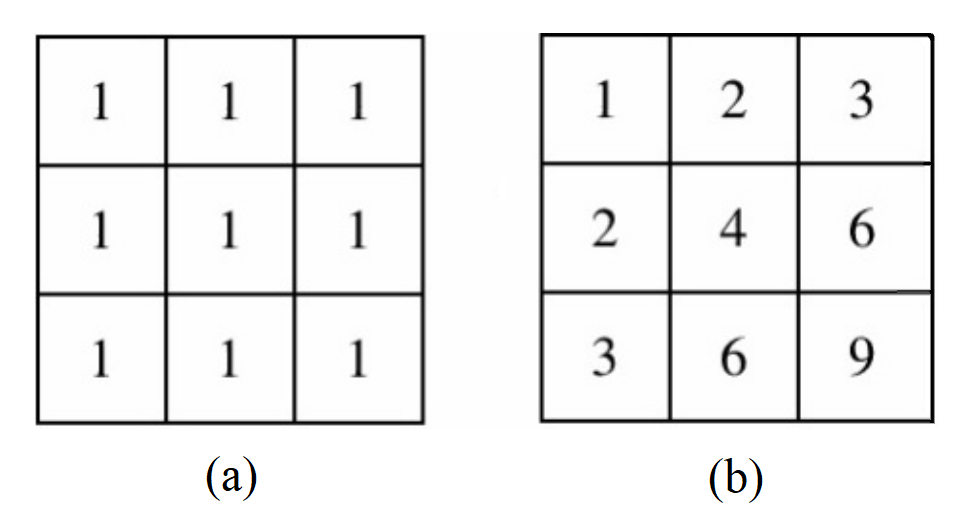
\includegraphics[width=0.5\textwidth]{Figures/integralImage.png}
	\caption{Výpočet integrálneho obrazu - vstupný obraz (A) , integrálny obraz (B)}
	\label{fig:integralImage}
\end{figure}


\begin{equation}
ii(x,y)=\sum_{x^{\prime}\leq x,y^{\prime}\leq y}i(x^{\prime},y^{\prime}),
\label{eq:integral}
\end{equation}


 Metóda funguje na porovnavaní celých blokov pixelov. Tieto bloky (častokrát nazývané aj zhluky) môžu mať rôzne tvary, veľkosť a natočenie. Tieto bloky môžu nadobúdať rôzne tvary ale vo všeobecnosti sa používajú 3 hlavné typy príznakov:
\begin{itemize}
  \item \textbf{Dvoj-obdĺžnikové} \textit{(angl. two-rectangle)} - porovnávajú sumu pixlov v obdĺžnikových oblastiach, ktoré sa nachádzajú vedľa seba, vodorovne, alebo zvislo.
  \item \textbf{Troj-obdĺžnikové} \textit{(angl. three-rectangle)} - porovnávajú sumu obdĺžnikových oblastí, ktoré sa nachádzajú po oboch stranách aktuálnej oblasti a sumu aktuálnej oblasti.
  \item \textbf{Štvor-obdĺžnikové} \textit{(angl. four-rectangle)} - počítajú rozdiel medzi dvoma aktuálnymi obdĺžnikovými oblasťami, ktoré sa dotýkajú svojimi rohmi a obdĺžnikovými oblasťami medzi nimi.
  
 \end{itemize}
   \begin{figure}[H]
	\centering
	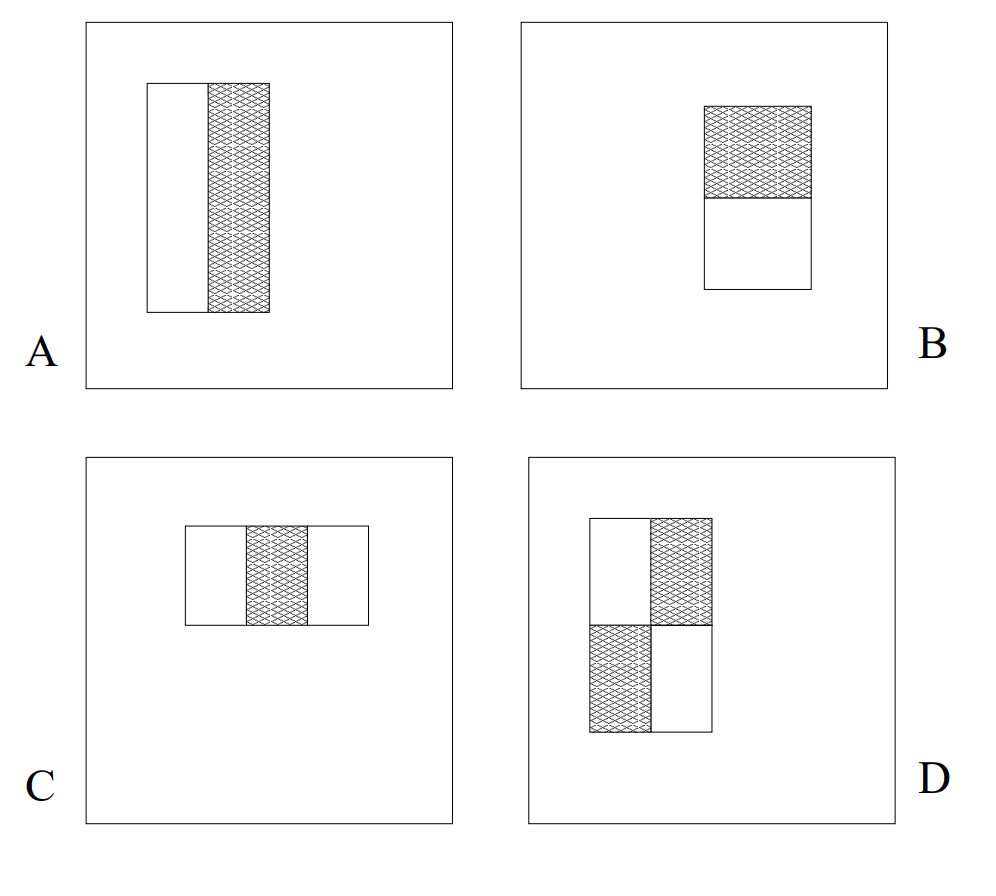
\includegraphics[width=0.6\textwidth]{Figures/haar1.png}
	\caption{Haar - dvoj-obdĺžnikové príznaky (A, B), troj-obdĺžnikové príznaky (C) a štvor-obdĺžnikové príznaky(D)\cite{viola2001robust}}
	\label{fig:Haar1}
\end{figure}
  Znázornenie jednotlivých typov príznakov môžeme vidieť na obrázku \ref{fig:Haar1}. Jednotlivé príznaky môžu byť použité pre rôzne typy obrázkov. Efektivita klesá pri použití príznaku na celý obraz. Vhodným riešením je preto skombinovať viacero príznakov. Na výber  správnych efektívnych príznakov sa používajú špeciálne algoritmy. Jedným z najpoužívanejších algoritmov  pre zvýšenie efektivity výberu príznakov je AdaBoost\cite{freund1995desicion}, ktorý vytvoril profesor Yoav Freund. Jedná se o klasifikačný algoritmus, ktorý je schopný vytvoriť dostatočne silný klasifikátor z kombinácii viacerých slabších klasifikátorov.  Metódou Haar je možné detekovať rôzne triedy objektov. Jedným z najčastejších a jednoducho detekovatelných  typov objektov je napríklad tvár.


\begin{figure}[H]
	\centering
	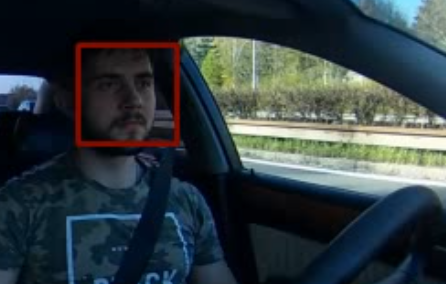
\includegraphics[width=0.6\textwidth]{Figures/haar2.png}
	\caption{Haar - detekcia tváre v slabých svetelných podmienkach}
	\label{fig:Haar2}
\end{figure}



\subsection{HOG}
\label{HOG}
S nápadom  vylepšiť detekciu objektov použitím príznakov prišli v roku 2005 Navneed Dalal a Bill Triggs \cite{dalal2005}, kde postupne vyskúšali niekoľko typov deskriptorov.  V práci taktiež podrobne rozobrali  možnosti a spôsoby ako správne určiť parametre ich detekčnej metódy pre správne fungovanie detekcie jednotlivých tried. Hlavnou myšlienkou ich metódy je, že objekt môže byť charakterizovaný  viacerými spôsobmi. Táto metóda je rozdelená do niekoľkých samostatných krokov (Obr. \ref{fig:HOG1}):
\begin{itemize}
  \item \textbf{Úprava obrazu} - v tomto kroku je potrebné  v obraze upraviť kontrast a jas, ktoré by mohli spôsobovať  problémy v nasledujúcich krokoch. Okrem tejto úpravy  je možné obraz upraviť napríklad gamma filtrom.
  \item \textbf{Výpočet gradientov} - veľkosť gradientov sa počíta na základe vstupného obrazu a masky. Masky, ktoré sa používaju v tomto kroku sú \textit{[-1, 0, 1]} alebo \textit{[-1, 0, 1] \textsuperscript{T}}. Gradienty je nutné vypočítať v obidvoch osách, čím sa získa \textit{I\textsubscript{x}} a \textit{I\textsubscript{y}}. Po získaní gradientov je potrebné vypočítať veľkosť gradientov \textit{m(x,y)} a ich smer \textit{$\theta(x, y)$}:
  
\begin{equation}
m(x,y)= \sqrt{I_{x}^{2} + I_{y}^{2}}
\label{eq:Výpočet veľkosti gradientu}
\end{equation}

  \begin{equation}
\theta(x, y) = \left(\frac{I_{y}}{I_{x}}\right)
\label{eq:Výpočet smeru gradientu}
\end{equation}
  \item \textbf{Normalizácia} -  pre správne fungovanie je potrebné obraz normalizovať, aby sa minimalizovali rozdiely medzi jednotlivými bunkami. Tento krok spočíva v skladaní viacerých buniek, čím následne vznikajú bloky. 
   \item \textbf{Deskriptor} -  je vytvorený zo vstupného obrazu do jednotlivých blokov. Jednotlivé bloky sa posúvajú a prekrývajú o daný počet pixelov. Výsledok deskriptoru je odovzdaný  klasifikátoru, ktorý následne určuje do akej triedy objekt patrí. Jeden z často používaných klasifikátorov je Support vector machine (SVM), ktorý napríklad používali autori vo svojej práci na efektívnu detekciu chodcov.\cite{pang2011efficient}
 \end{itemize}


\begin{figure}[H]
	\centering
	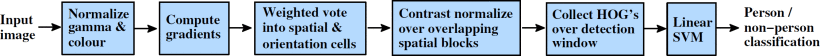
\includegraphics[width=1\textwidth]{Figures/hog.png}
	\caption{HOG - séria krokov \cite{dalal2005}}
	\label{fig:HOG1}
\end{figure}

Výstupom tejto metódy je množina histogramov pre jednotlivé bloky. Histogram predstavuje grafické rozloženie intenzity jasu vstupného obrazu. Pri niektorých špecifických obrazoch je potrebné histogram vyrovnať. Tento krok je potrebný najmä pri obrazoch, ktoré su príliš tmavé alebo príliš svetlé. Pomocou vyrovnania \textit{(angl. equalization)} histogramu  dokážeme zvýšiť kontrast obrazu. Jednotlivé kroky znázornené na vstupnom obraze chodca môžeme vidieť na obrázku \ref{fig:HOG2}\par


\begin{figure}[H]
	\centering
	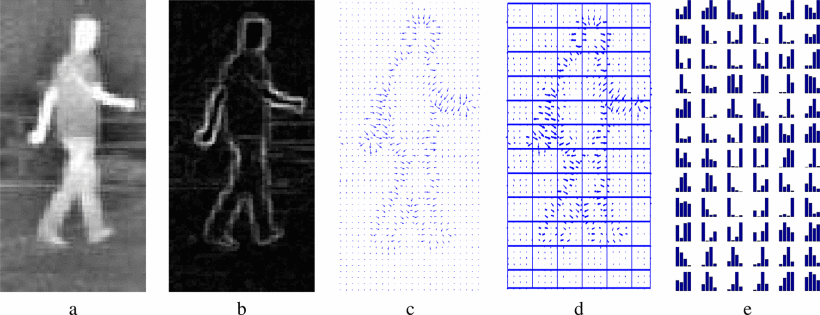
\includegraphics[width=1\textwidth]{Figures/hog3.png}
	\caption{HOG - vstupný obraz (a), normalizácia gradientu (b), orientácia gradientu (c), rozdelenie do buniek (d) vypočítané histogramy (e). \cite{bertozzi2007pedestrian}}
	\label{fig:HOG2}
\end{figure}


\newpage
\subsection{OpenPose}
OpenPose\cite{cao2018openpose} je framework, ktorý bol prvýkrat uvedený verejnosti už v roku 2016. Detekcia ľudského postoja predstavuje hlavný problém s lokalizáciou častí ľudského tela ako sú ramená, lakte a členky zo vstupného obrázka alebo videa. Vo väčšine dnešných aplikácií detekcie postáv v reálnom svete sa vyžaduje vysoký stupeň presnosti, ako aj spracovanie v reálnom čase.
OpenPose, ktorý bol vyvinutý výskumníkmi na univerzite Carnegie Mellon University, možno považovať za najmodernejší prístup pri detekcii ľudských v reálnom čase. Jedná sa o open-source projekt, ktorého zdrojové kôdy sú verejne dostupné\cite{githubOpenpose}.

\begin{figure}[H]
	\centering
	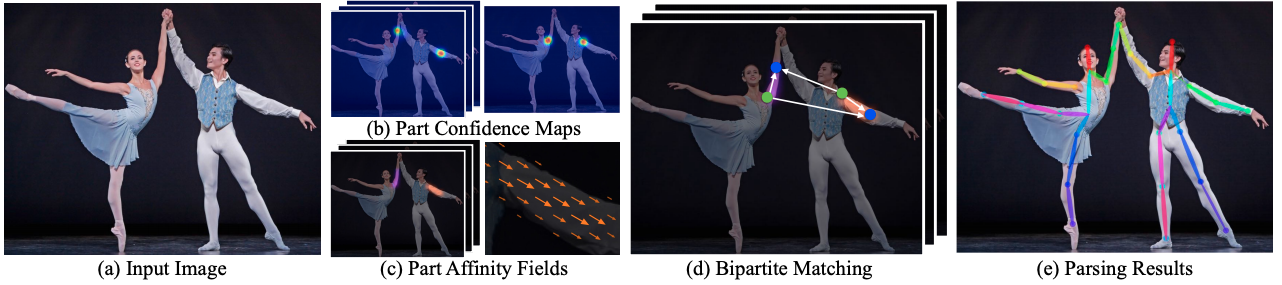
\includegraphics[width=1\textwidth]{Figures/openposePipeline.png}
	\caption{OpenPose - odhad viacerých ôsob v reálnom čase pomocou polí afinity filtra.\cite{cao2018openpose}}
	\label{fig:openposeOverall}
\end{figure}

 Samotný framework je veľmi detailne vysvetlený a dobre zdokumentovaný. OpenPose bol pôvodne napísaný v C++ a Caffe\cite{jia2014caffe}. Postupom času však  autori vytvorili aj  nadstavbu pre jazyk Python, s ktorým sa rozšírili možnosti jeho využitia medzi ostatnými programátormi. Základná myšlienka detekcie pomocou OpenPose sa skladá z viacerých krokov:

\begin{itemize}
\item \textbf{Spracovanie vstupného obrazu} - vstupný obrázok (Obr. \ref{fig:openposeOverall}a) privádza ako vstup do dvojvetvovvej viacstupňovej Konvolučnej nerónovej siete (CNN). Dve vetvy znamenajú, že CNN produkuje dva rôzne výstupy z jedného vstupného obrazu. Viacstupňové znamená, že sieť je v každej fáze naskladaná jedna na druh. Tento krok je analogický jednoduchému zväčšeniu hĺbky neurónovej siete s cieľom zachytiť podstatnejšie výstupy smerom k posledným stupňom.

\item \textbf{Spracovanie v dvoch vetvách} - prvá vetva predpovedá mapy dôveryhodnosti (Obr. \ref{fig:openposeOverall}b) rôznych častí tela, ako je pravé oko, ľavé oko, pravé lakte a podobne. Druhá vetva zobrazená modrou farbou predpovedá afinitné polia (Obr. \ref{fig:openposeOverall}c), čo predstavuje stupeň asociácie medzi rôznymi časťami tela.

\item \textbf{Viacfázové spracovanie} - v prvej fáze sieť vytvorí počiatočnú sadu detekčných máp spoľahlivosti \textit{S} a množinu polí afinity častí \textit{L}. Potom v každej nasledujúcej fáze predpovede z obidvoch vetiev v predchádzajúcej fáze, spolu s pôvodnými obrazovými znakmi \textit{F}, sú zreťazené a použité na vytvorenie podrobnejších predpovedí. Pri implementácii OpenPose sa posledná fáza \textit{t} zvolí ako číslo 6.
\end{itemize}

\subsubsection{Mapa spoľahlivosti}
Prvá vetva v neurónovej sieti OpenPose vytvára sadu máp spoľahlivosti \textit{S} (rovnica \ref{eq:confidencemap}). V podstate sa jedná o tabuľku, v ktorej je každej časti tela z datasetu priradená miera spoľahlivosti v rozsahu 0 až 1. 

\begin{eqnarray}
& S = (S_{1}, S_{2}, S_{3} ... S_{j}) \label{eq:confidencemap}\\
& S\in\mathbb{R}^{w \times  h},\nonumber\\
& j\in \left \{1,\: J  \right \}, kde\: J\: je\: počet\: všetkých\: častí\: tela\nonumber
\end{eqnarray}
Počet častí tela závisí od množiny datasetov, s ktorými je program OpenPose trénovaný. Pokiaľ ide napríklad o súbor datasetu COCO\cite{lin2014microsoft}, \textit{J = 19}, pretože existuje 18 rôznych kľúčových bodov tela + 1 pozadie. Obrázok \ref{fig:cocoDataset} znázorňuje rôzne časti tela s prideleným identifikátorom pre súbor údajov COCO. Pre model trénovaný s dátovým súborom COCO bude sada \textit{S} obsahovať prvky \textit{S1, S2, S3,…, S19}. V tomto príklade predpokladáme, že prvok \textit{S1} zodpovedá mape spoľahlivosti pre kľúčový bod s číslom 0, ktorý zodpovedá nosu (Obr. \ref{fig:cocoDataset}).\par. Ako jednoduchý príklad môže poslužiť predstava, že celý obraz má šírku a výšku 5px, čo vedie k vytvoreniu  mapy spoľahlivosti o veľkosti \textit{$5\times 5$}. Vo vstupnom obrázku sa nachádza iba jedna tvár. Preto pre mapu spoľahlivosti \textit{S1} (zodpovedajúca za detekciu nosa) je možné vidieť hodnoty s vysokou spoľahlivosťou iba v oblasti, kde sa nos nachádza.\bigskip

\begin{figure}[H]
	\centering
	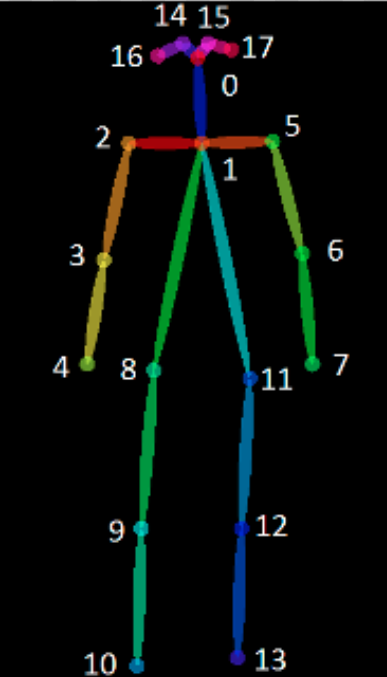
\includegraphics[width=0.3\textwidth]{Figures/cocoDataset.png}
	\caption{COCO - označenie častí tela v COCO datasete.\cite{cocoDataset}}
	\label{fig:cocoDataset}
\end{figure}


\subsubsection{Part afinity fields (PAF)}
Druhá vetva neurónovej siete vytvára množinu čiastkových afinitných polí \textit{L} (rovnica \ref{eq:pafmap}).

\begin{eqnarray}
& L = (L_{1}, L_{2}, L_{3} ... L_{c}) \label{eq:pafmap}\\
& L\in\mathbb{R}^{w \times  h \times 2},\nonumber\\
& c\in \left \{1,\: C  \right \}, kde\: C\: je\: počet\: všetkých\: končatín\nonumber
\end{eqnarray}

Celkový počet končatín a párov závisí od datasetu, s ktorým je OpenPose trénovaný. Kvôli prehľadnosti sa uvádzajú dvojice častí tela ako končatiny, napriek tomu, že niektoré páry častí tela nie sú v skutočnosti končatinami (Napríklad oko-nos, ucho-oko atď.). Pre dataset COCO je počet párov končatín, \textit{C = 19}. Môžeme si predstaviť, že každý prvok v množine \textit{L} je mapa veľkosti \textit{$w\times h$}, kde každá bunka obsahuje 2D vektor predstavujúci smer párových prvkov. Napríklad na obrázku \ref{fig:cocoDataset} je možné vidieť, že pár častí tela pozostáva z pravého ramena k pravému laktu. Schéma potom ukazuje smerový vektor, ktorý ukazuje z pravého ramena na pravý lakeť. Celý zoznam párov končatín je znázornený vo výpise \ref{src:coco_pairs}.\bigskip

\begin{lstlisting}[language=Python,label=src:coco_pairs,caption={Množina párov končatín v datasete COCO}]
COCO_PAIRS = [(1, 2), (1, 5), (2, 3), (3, 4), (5, 6), (6, 7), (1, 8), (8, 9), (9, 10), (1, 11), (11, 12), (12, 13), (1, 0), (0, 14), (14, 16), (0, 15), (15, 17), (2, 16), (5, 17)]
\end{lstlisting}

\bigskip
Okrem Datasetu COCO Dokáže OpenPose pracovať aj s mnohými ďalšími datasetmi. OpenPose bol skúšaný a trénovaný napríklad s datasetmi MPI\cite{andriluka14cvpr}, BODY\_25 alebo BODY\_25b. Datasety sa líšia vo veľkosti, rýchlosti, ale napríklad  aj v presnosti samotnej detekcie. Jednotlivé datasety majú medzi sebou nasledujúce rozdiely:


\begin{itemize}
\item \textbf{COCO} - starší dataset, na ktorom bol OpenPose pôvodne vyvíjaný. Postupne sa však nahradzuje novými a modernejšími datasetmi. Jeho výhodou je, že vyžaduje menej pamäte na GPU (schopnosť pracovať s 2 GB GPU a predvoleným nastavením) a pri režíme CPU pracuje rýchlejšie oproti novšiemu BODY\_25.

\item \textbf{BODY\_25} - jedná sa o novší dataset, ktorý je rýchlejší, presnejší a obsahuje ďalšie trénovacie dáta k častiam tela, ktoré nie sú obsiahnuté v COCO datasete ako napríklad chodidlá. Jeho nevýhodou sú hlavne vysoké hardwarové nároky.

\item \textbf{MPI} - je určený pre ľudí, ktorí požadujú štruktúru datasetu MPI. Je tiež pomalší oproti BODY\_25 a oveľa menej presný.
\end{itemize}




\newpage
\subsection{TF Pose Estimation}
Tento framework pre detekciu postáv bol implementovaný pomocou knižnice Tensorflow. Poskytuje tiež niekoľko variantov, ktoré sa odlišujú najmä v zmenách pre spracovanie v reálnom čase na CPU alebo zariadení s nízkou spotrebou. Z tohto dôvodu ho je  možné používať napríklad na mobilných zariadeniach alebo internetových prehladiačoch použitím knižnice tensorflow.js. Tensrflow Pose estimation používa na detekciu  vlastný model s názvom PoseNet. PoseNet sa dá použiť na odhad jednej pozície alebo viacerých pozícií v obraze súčasne. To znamená, že existuje verzia algoritmu, ktorý dokáže detekovať iba jednu osobu v obraze a druhá verzia, ktorá dokáže zistiť viac osôb v obraze. Hlavnou výhodou použitím detekcie jednej osoby je rýchlejšie spracovanie a nižší výpočtový výkon. Podstatnou nevýhodou však je, že vyžaduje iba jeden objekt prítomný na obrázku. Pri súčasnej pozícii viacerých osôb v obraze tento algoritmus nedokáže zdetekovať správne ani jednu osobu. Je preto potrebné sa zamyslieť sa  hneď na začiatku, koľko ôsob sa reálne môže v obraze nachádzať. Hlavná myšlienka tohto algoritmu sa skladá z dvoch krokov podobne ako pri knižnici OpenPose.

\begin{itemize}
\item \textbf{Detekcia pozície} - na najvyššej úrovni modelu PoseNet sa vráti objekt, ktorá obsahuje zoznam kľúčových bodov a skóre spoľahlivosti pre každú detekovanú osobu.
\item \textbf{Výpočet spoľahlivosti pozície} - skóre spoľahlivosti určuje celkovú dôveru v odhadovaní pozície. Je v rozsahu od 0 až 1. Môže sa použiť na skrytie pozícií, ktoré sa nepovažujú za dostatočne výrazné.
\item \textbf{Výpočet kľúčových bodov} - odhadované časti tela osoby, ako napríklad nos, pravé ucho, ľavé koleno, pravá noha atď. Obsahuje pozíciu a spoľahlivosť kľúčového bodu. PoseNet štandardne zisťuje 17 kľúčových bodov.
\item \textbf{Poloha kľúčového bodu} - pozostáva z 2D súradníc v pôvodnom vstupnom obrázku, kde bol zistený kľúčový bod.
\end{itemize}


Model PoseNet je nezávislý na veľkosti vstupného obrazu. To znamená, že môže predikovať polohy pozícií v rovnakom rozlíšení ako pôvodný obrázok bez ohľadu na to, či je obraz zmenšený. PoseNet môže byť nakonfigurovaný tak, aby mal vyššiu presnosť na úkor rýchlosti detekcie nastavením výstupného kroku. Výstupný krok určuje, do akej miery zmenšujeme výstup vzhľadom na veľkosť vstupného obrázka. To ovplyvňuje veľkosť jednotlivých vrstiev a výstupy modelu. Čím vyšší je výstupný krok, tým menší je počet vrstiev v sieti a výstupoch a tým aj ich presnosť. V základnej implementácii môže mať výstupný krok hodnoty 8, 16 alebo 32. Inými slovami, výstupný krok 32 bude mať za následok najrýchlejší výkon, ale najnižšiu presnosť, zatiaľ čo 8 bude mať najvyššiu presnosť, ale najpomalší čas detekcie.


\subsubsection{Výstup}
Keď PoseNet spracováva obraz, v skutočnosti vytvára tepelnú mapa \textit{(angl. Heatmap)} spolu s ofsetovými vektormi, ktoré je možné dekódovať, aby sa v obraze našli oblasti s vysokou spoľahlivosťou. Veľkou výhodou pri detekcii postáv v obraze cez Tensorflow je teda to, že spolu s vektormi výstupného modelu dostávame aj štruktorované dáta pravdepodobnosti jednotlivých častí postavy, ktoré môžeme využiť na ďalšie spracovanie, alebo znázorniť pre lepšiu predstavu\textit{(Obr. \ref{fig:tfPoseHeatmap})}.

\subsubsection{Tepelná mapa}
Každá pozícia v tejto tepelnej mape má určité skóre spoľahlivosti. Tento údaj vyjadruje pravdepodobnosť, že v danom umiestnení existuje určitá časť daného typu. Dá sa to považovať za rozdelenie pôvodného obrázka do mriežky \textit{$15\times 15$}, kde skóre v termografickej mape poskytuje klasifikáciu pravdepodobnosti, že každý kľúčový bod existuje v každom štvorci mriežky.

\subsubsection{Výstupný vektor}
Každý výstupný vektor je 3D vektor, ktorý má veľkosť \textit{$šírka  \times výška \times 34$}. Číslo 34 je dvojnásobok kľúčových bodov( 2 $\times$ 17). Tepelné mapy sú iba aproximáciou toho, kde sa skutočné kľúčové body nachádzajú, pričom výstupné vektory zodpovedajú svojou polohou bodom tepelnej mapy a používajú sa na predpovedanie presnej polohy jednotlivých častí ľudského tela. Prvých 17 rezov výstupného vektora obsahuje x-ovú súradnicu vektora a posledných 17 rezov y-ovú súradnicu. Veľkosti výstupného vektora sú v rovnakej mierke ako pôvodný vstupný obrázok.

\begin{figure}[H]
	\centering
	\includegraphics[width=1\textwidth]{Figures/tfPose1.png}
	\caption{Tepelná mapa  - vstupný obraz (a), tepelná mapa postavy (b)}
	\label{fig:tfPoseHeatmap}
\end{figure}

\subsection{AlphaPose}
AlphaPose\cite{fang2017rmpe} je framework, ktorý vznikol v roku 2017. Je zameraný na detekciu ľudských postáv v najpresnejšej miere. Tento framework pracuje na princípe používania ohraničovacích boxov \textit{(angl. bounding box)}. Pre efektívne fungovanie algoritmu je použitý najmodernejší detektor objektov. Autori práce použili natrénovaný model Faster RCNN\cite{ren2015faster} a model pre detekciu postáv v obraze\cite{newell2016stacked}, ktorý je zameraný na SPPE detekciu. Primárna myšlienka práce spočíva v riešení dvoch hlavných problémov, ktoré pri takejto detekcii vznikajú:
\begin{itemize}
\item \textbf{Problém lokalizačnej chyby} - skutočnosti je tento model dosť náchylný na chyby pri spočívajúce v použití ohraničovacích boxov. Aj v prípadoch, keď sú ohraničovacie rámčeky
sú považované za správne a majú dostatočne vysokú spoľahlivosť \textit{$(I_oU > 0,5)$}, zistené ľudské pozície môžu byť stále nesprávne. 
\item \textbf{Redundantná detekcia} - model vytvára pózu pre každý ohraničovací box, čo vo výsledku vedie k duplicitnej detekcii rovnakej osoby (Obr. \ref{fig:alphaPoseRedundant})
\end{itemize}

\begin{figure}[H]
	\centering
	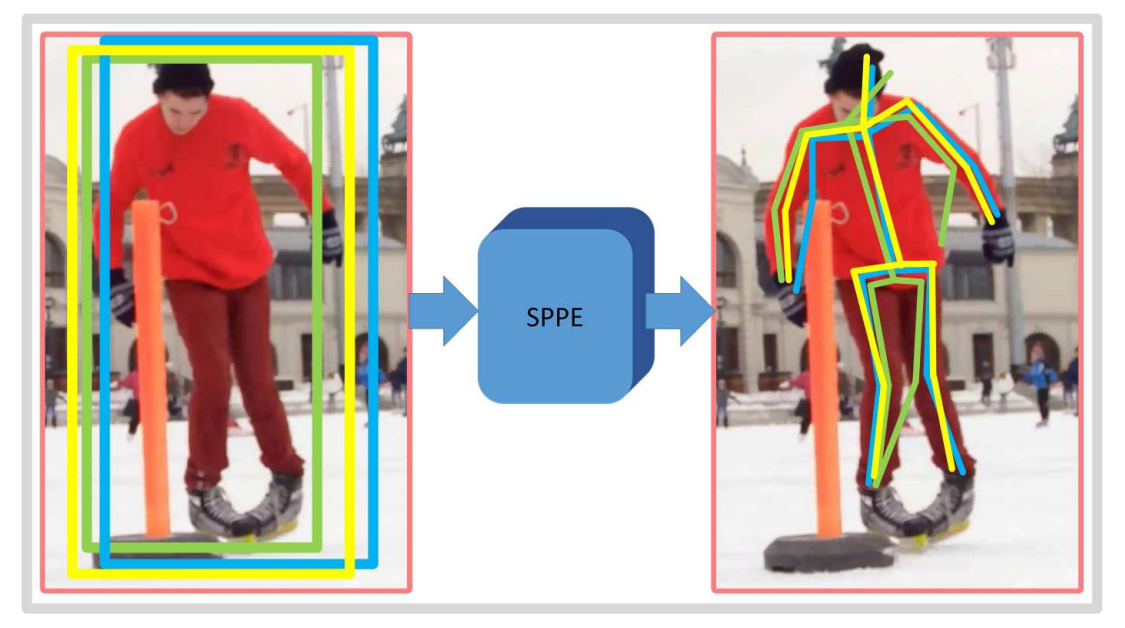
\includegraphics[width=0.6\textwidth]{Figures/alphaPoseRedundant.png}
	\caption{Problém redundantnej detekcie s použitím metódy bounding box\cite{fang2017rmpe}}
	\label{fig:alphaPoseRedundant}
\end{figure}

Na vyriešenie uvedených problémov je použitý model na regionálnu detekciu viacerých postáv (RMPE). Vďaka tomu
framework vylepšuje výkon algoritmov na odhadovanie ľudských postojov založených na modeli SPPE. Autori práce tiež navrhli novú symetrickú sieť pre priestorovú detekciu (SSTN), ktorá je pripojená k SPPE na extrakciu jednotlivej osoby z
oblasti nepresného ohraničovacieho boxu. Na optimalizáciu tejto siete je zavedená ďalšia paralelná vetva SPPE. Na riešenie problému redundantnej detekcie, je použitý parametrický NMS, ktorý eliminuje nadbytočné pózy pomocou novej metriky vzdialenosti a porovnanie podobnosti pózy. Prístup založený na údajoch je
aplikovaný na optimalizáciu parametrov metriky vzdialenosti. RMPE je navrhnutý veľmi všeobecne a práve vďaka tomu je použiteľný pre rôzne ľudské detektory a ďalšie knižnice, ktoré pracujú na princípe single-person detection. AlphaPose používa dataset MPII, s ktorým prekonáva najmodernejšie metódy ako OpenPose. Tento model a zdrojové kódy\cite{githubAlphaPose} sú verejne dostupné a určené primárne pre vedu a výskum.

\newpage
\subsection{Ostatné metódy}
Okrem  najpoužívajenších metód ako OpenPose, TF pose estiamtion, či AlphaPose existuje aj mnoho ďalších riešení. Tieto riešenia často vychádzajú zo základného princípu detekcie postáv, ktoré používajú aj tieto hlavné knižnice. Hlavný rozdiel je však použitie upravenej neurónovej siete alebo zmena rôznych parametrov. Vďaka takejto úprave je možné dosiahnúť v špecifických prípadoch vyššiu úspešnosť a presnosť detekcie alebo dokonca znížiť výpočtový čas potrebný na detekciu a spracovanie. Tieto riešenia sú však často obmedzované najmä chýbajúcou dokumentáciou, nedostatočnou implementáciou vo viacerých jazykoch, alebo nemožnosťou jednoduchej zmeny konfigurácie. Okrem voľne dostupných riešení existuje aj mnoho projektov, ktoré nemajú verejné zdrojové kódy a slúžia len pre komerčné použitie, čo môže mnoho používateľov zo začiatku odradiť. Jedným z takýchto projektov je napríklad WrnchAI, ktorému je venovaná nasledujúca podkapitola.


\subsubsection{WrnchAI}
WrnchAI je framwork, ktorý bol vytvorený už v roku 2014. S myšlienkou využiť umelú inteligenciou a založiť projekt pre detekciu postáv prišiel Paul Kruszewski. Napriek tomu, že tento framework  existuje už niekoľko rokov a v niektorých článkoch\cite{openposeVsWrnchAI} dokázal dokonca získať lepší čas detekcie oproti iným metódam,  nestal sa veľmí populárnym medzi vývojarmi. Jedným z hlavných dôvodov je to, že knižnica nie je voľne dostupná pre vývojárov a jedná sa o platený projekt bez voľného prístupu k zdrojovému kódu. Súčasná cenová politika základnej verzie sa pohybuje na úrovni \$500 za mesiac používania s možnosťou vyskúšania trial verzie na prvý mesiac zadarmo. Trial verzia však funguje v obmedzenom režime  bez prístupu ku všetkým platformám. Pre bežného človeka sa táto cena môže zdať privysoká, avšak vzhľadom na jeho široké možnosti využitia  v rôznych oblastiach sa jedná o adekvátnu cenu. WrnchAI však našiel svoje uplatnenie možnosťou využitia na rôznych typoch zariadení, ktoré sa prispôsobujú konkrétnym podmienkam. V súčasnosti WrnchAI poskytuje 4 hlavné platformy:
\begin{itemize}
\item \textbf{wrnchPC} - umožňuje zachytiť ľudský pohyb neobmedzeného množstva ľudí, bez toho, aby boli použité drahé senzory či kamery. WrnchPC je postavený na základoch  umelej inteligencie tak, aby sa ľahko integroval do všetkých aplikácií. Použité sú modely hlbokého učenia, aby bolo zabezpečené spoľahlivé zachytenie ľudského pohybu pre všetky činnosti a v akomkoľvek prostredí.


\item \textbf{wrnchCloud} - detekuje ľudský postoj na vzdialenom serveri. WrnchCloud je nákladovo veľmi efektívne riešenie, pretože nepotrebuje žiadne vysoké hardwarové nároky okrem bežného počítača s pripojením na internet. Celý proces detekcie prebieha na serveri, čo odľahčuje zákaznika od nákupu drahých grafických kariet a iného hardwaru. Toto riešenie je škálovateľné s možnosťou spracovania viacerých vstupov súčasne. Využitie cloudového riešenie zároveň pomáha držať krok moderných trendov v internetových technológiách.

\item \textbf{wrnchMobile } - umožňuje využiť mobilné zariadenia na vytvorenie programu snímania postáv v reálnom čase. Taktiež dokáže spolupracovať s mobilnými operačnými systémami ako Android alebo IOS. Jeho základnym princípom je efektívne využitie výpočtového výkonu  na malých prenosných zariadeniách ako sú napríklad mobilné telefóny. Tento druh platformy taktiež dokáže pracovať aj s dalšími pokročilými vecami ako je napríklad rozšírená realita. S touto pomocou rozšírenej reality dokáže wrnchMobile snímanú postavu detekovať a zároveň zobrazovať napríklad do VR okuliarov.


\item \textbf{wrnchEmbedded} - poskytuje možnosť detekovať postavy na rôznych automatizovaných zariadeniach ako napríklad roboty, samoriadiace vozidlá, aby mohli v reálnom čase vidieť a interagovať s ľuďmi a ich pohybom. WrnchEmbedded pomáha zariadeniam predvídať ľudské správanie a najlepšie reagovať vo všetkých situáciách. Ich program je optimalizovaný najmä na rôzne priemyselné platformy a počítače, vďaka ktorým by mala byť ich integrácia s platformou Wrnch veľmi jednoduchá. V súčasnosti je však táto časť platformy stále v aktívnom vývoji a momentálne nie je dostupná. 
\end{itemize}

\begin{figure}[H]
	\centering
	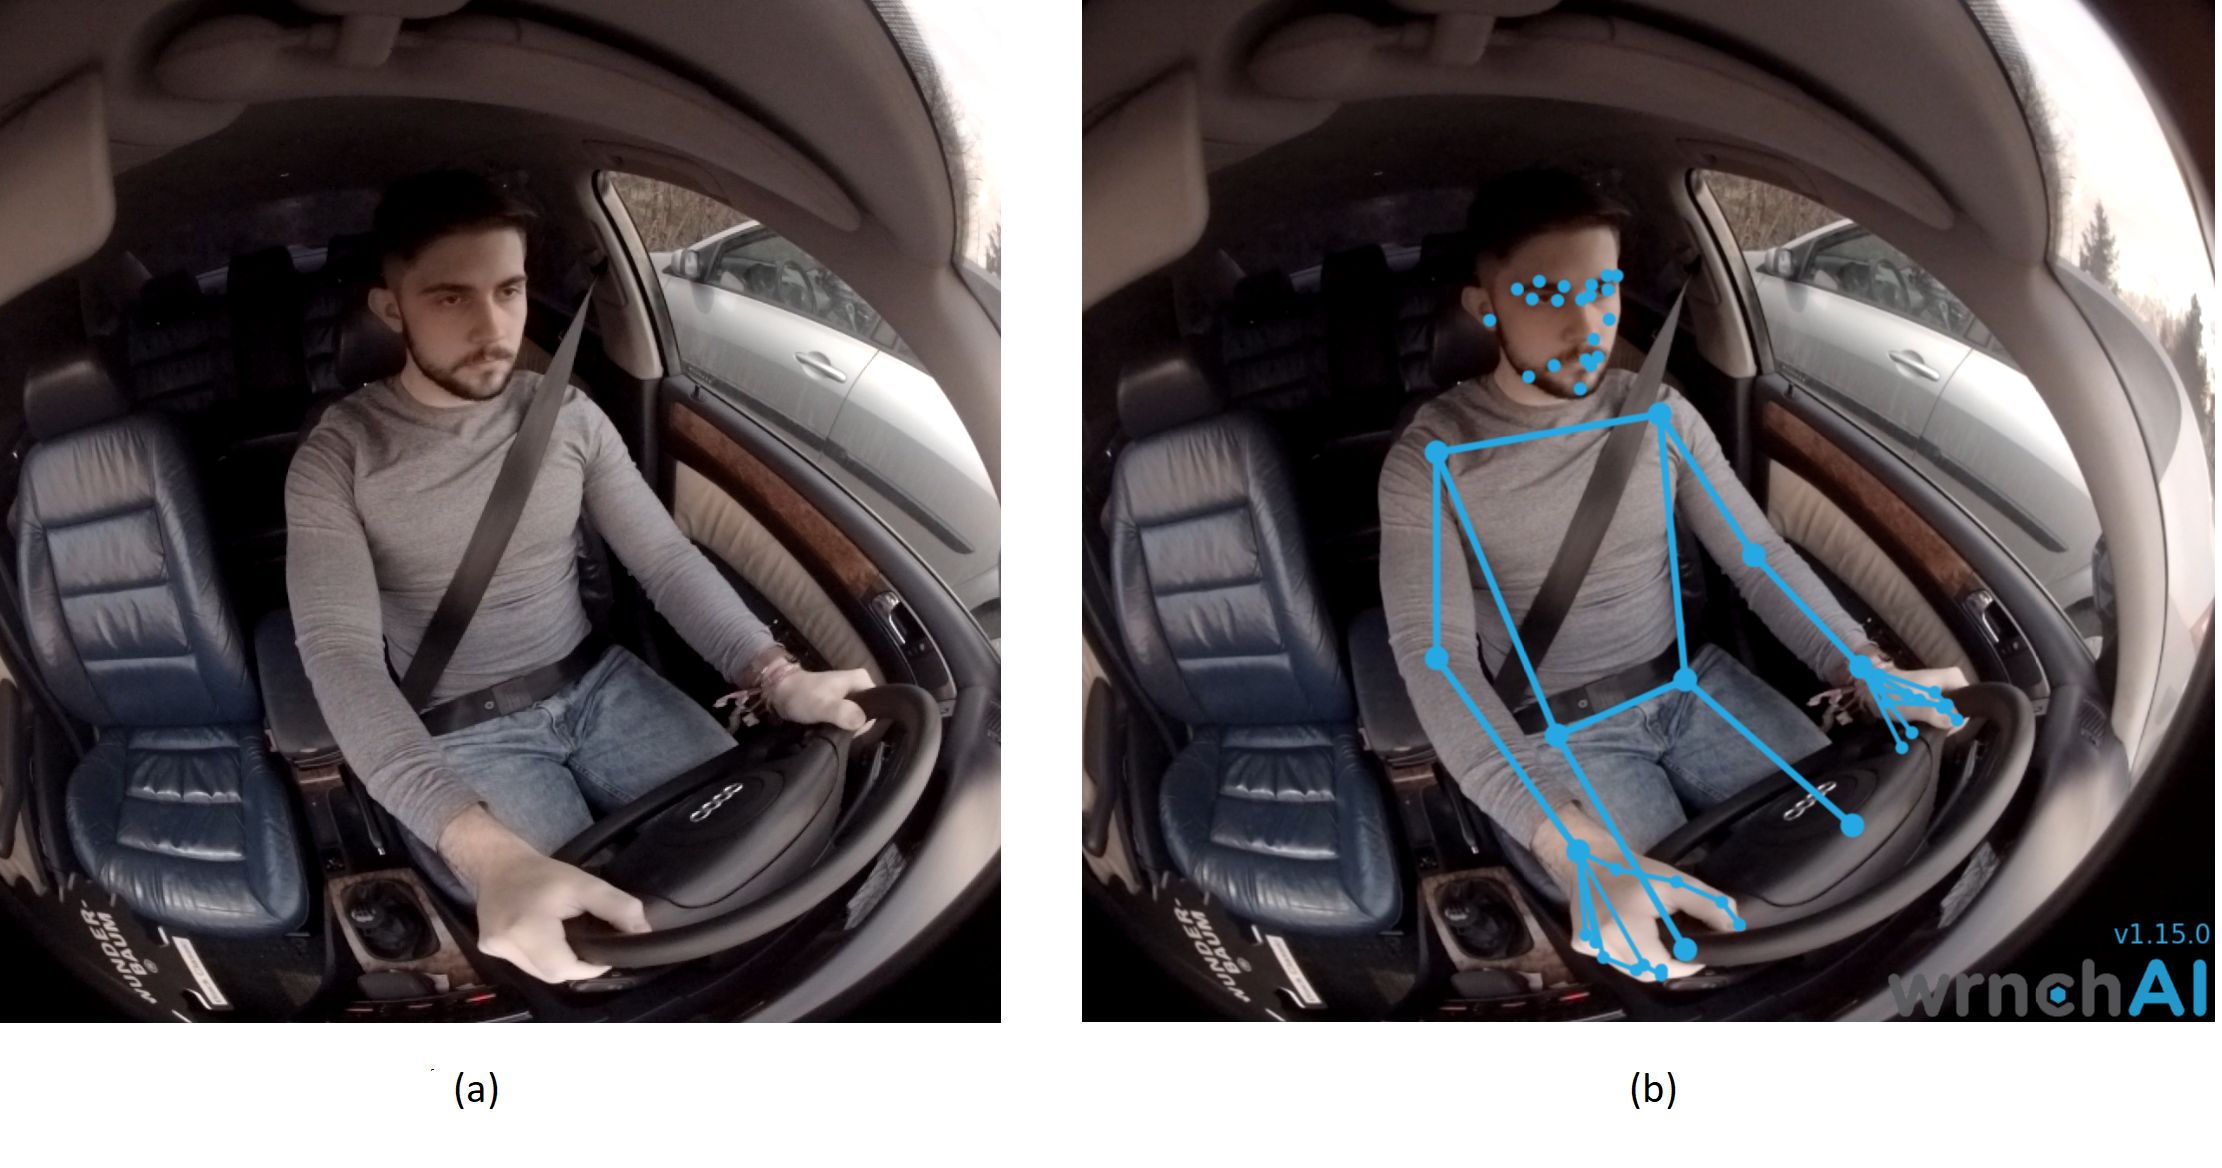
\includegraphics[width=0.9\textwidth]{Figures/wrnchAI.png}
	\caption{WrnchAI - vstupný obraz (a), výsledok spracovania na platforme WrnchCloud(b)}
	\label{fig:wrnchAICloud}
\end{figure}

Na obrázku \ref{fig:wrnchAICloud} môžeme vidieť výsledok metódy cloudovej platformy WrnchAI. Táto platforma  funguje dostatočne spoľahlivo aj pri atypických polohách ľudského tela, ako je napríklad sedavá poloha vodiča za volantom. WrnchAI okrem polohy tela poskytuje aj detekciu kľúčových bodov tváre a kľúčové body rúk a prstov. Oproti ostatným knižniciam a frameworkom je možnost použiť WrnchAI ako komplexné riešenie na detekciu celého ľudského tela, čo napríklad pri OpenPose nie je bez použitia dalších rozšírení možné. V skúšobnej trial verzii  taktiež nie je možné odstrániť vodoznak firmy, ktorý sa nachádza v pravom dolnom rohu výstupného obrázka.


\newpage
\section{Detekcia vodiča vo vozidle}
\label{sec:Pose detection}
Hlavným zmyslom detekcie vodiča je analyzovanie jeho správania za volantom.  Pomocou takejto analýzy dokážeme napríklad odhadnúť, či je vodič unavený, alebo či sa dostatočne venuje okolitej premávke. Detekcia vodiča vo vozidle môže byť vykonaná viacerými spôsobmi. Zariadenie, ktoré sleduje vodičovo správanie môže byť založené na rôznych mechanických alebo digitálnych senzoroch, či kamerách. Aby sa zamedzilo zlyhaniu celého systému a nesprávnemu vyhodnoteniu situácie, je vhodné kombinovať viacero takýchto systémov vo vozidle sučasne. Existujú systémy, ktoré dokážu analyzovať správanie vodiča pomocou reakcie na točenia volantom, alebo rôzne trhavé reakcie vodičovho tela, ktoré sú spôsobené pokročilou fázou mikrospánku. Táto fáza je však už často sprevádzaná ďalšími príznakmi, ako zatvorenie očí a  krátkodobé nevnímanie situácie, čo môže byť veľmi nebezpečné pre vštkých účastníkov premávky.  Okrem toho je možné snímať napríklad  vodičove oči pomocou digitálnej kamery. Systém by mohol vyhodnocovať  pravidelnosť mrknutia očí a na základe celej trasy odhadnúť úroveň únavy. Aby bol systém dostatočne spoľahlivý mal by mať nasledujúce vlastnosti:
\begin{itemize}
\item \textbf{Okamžitá detekcia} - každý systém musí byť dostatočne rýchly a schopný zdetekovať nepozornosť alebo mikrospánok vodiča maximálne behom 1-2 sekúnd. Každá sekunda navyše v rýchlo idúcom vozidle dramaticky zvyšuje riziko vzniku dopravnej nehody.
\item \textbf{Fungovanie v zhoršených podmienok} - systém by  fungovať vo všetkých podmienkach  spoľahlivo. Nemal by byť obmedzený zhoršenými svetelnými podmienkami, alebo napríklad vodičovými nepravidelnými pohybmi, ktoré sa môžu podobať na mikrospánok.
\item \textbf{Upozornenie} - pre úspešné fungovanie systému je požadujúce, aby dokázal nielen detekovať problém s vodičom, ale aj účinne zabrániť následkom vzniknutej situácie. To je možné vykonať napríklad hlasným zvukovým upozornením , prípadne spomalením až zastavením vozidla v prípade väčšieho problému s vodičovým vedomím. 
\end{itemize}
Samotná detekcia obrazu v uzavretom priestore sa od bežnej detekcie v základných princípoch nelíši. Obmedzenia nastávajú najmä nevhodnou pozíciou alebo natočením kamery, ktorá je umiestnená vo vozidle. Ak je kamera nesprávne umiestnená, alebo má nedostatočný uhol záberu, nemusí byť zdetekovaný celý snímaný objekt, čo môže viesť k chybe pri jeho detekcii. Autori v práci na analýzu vodiča \cite{smith2003determining}, kde sa zameriavali na oblasť tváre vodiča použili kameru umiestnenú v oblasti stredu palubnej dosky. Tým dosiahli takmer priame natočenie kamery na vodiča, bez toho, aby ho táto kamera výraznejšie obmedzovala vo výhľade. Keďže táto práca bola zameraná primárne na detekciu očí a úst, nebolo potrebné  používať kameru s vysokým uhlom záberu. Celý proces snímania však nebol spracovaný v reálnom čase, ale až po presune a spracovaní nahratých videí z kamery. Aby sa dal použiť takýto systém aj v reálnej premávke, bolo by potrebné aby dokázal spracovávať video  a vyhodnocovať vodičovo správanie v reálnom čase. Jedným z takýchto riešení by mohlo byť napríklad použitie malej priemyselnej kamery spolu s počítačom.\par
Zariadenie na detekciu ospalosti vodiča  ponúka aj celosvetová firma Bosch. Ich detekcia ospalosti vodiča je založená na algoritme, ktorý začína zaznamenávať správanie vodiča pri začatí jazdy. Vyrobca si však uvedomoval všetky nedostatky použitia kamery na smínaie a preto sa rozhodol vymyslieť detekciu  spánku iným spôsobom. Na volante je pripevnené špeciálne zariadenie, ktoré sníma otáčanie volantom. Následne rozpoznáva zmeny v priebehu dlhých ciest a tým pádom aj únavu vodiča. Typickými znakmi klesajúcej koncentrácie sú fázy, počas ktorých vodič sotva riadi, v kombinácii s miernymi, ale rýchlymi a prudkými pohybmi volantu, aby udržal vozidlo na ceste. Takéto riešenie však môže byť limitujúce, pretože nedokáže na mikrospánok zareagovať okamžite. Z tohto dôvôdu ho firma Bosch predáva hlavne ako pomocný systém na odhalenie únavy vodiča. \par
Mnoho podobných riešení zameraných na snímanie aktivity vodiča sa snažia zaviesť aj výrobcovia automobilov. Títo výrobcovia si veľmi dobre uvedomujú, že veľká časť dopravných nehôd býva spôsobená mikrospánkom, alebo len nepozornosťou vodiča. Príkladom môže byť vyrobca automobilov značky BMW, ktorý vo svojich vozidlách ponúka ako príplatkovú výbavu kameru na snímanie správania vodiča. Táto kamera dokáže reagovať napríklad na únavu alebo zatvorenie očí vodiča. Vo všeobecnosti tento systém dokáže dokonca reagovať aj na to, že vodič má otočenú hlavu a nesleduje premávku, čo môže viesť k nebezpečnej situácii. V každom takomto prípade je vodič upozornenený zvukovým znamením. Kamera je umiestnená v prístrojovej doske na mieste za volantom, odkiaľ je na tvár vodiča priamy výhľad (obr. \ref{fig:bmwAssistent}). Okrem jej vhodného umiestnenia je navyše vybavená aj IR LED diódami, vďaka ktorým kamera funguje aj za znížených svetelných podimenok a v noci, kedy sa vyskytuje najväčší počet mikrospánkov u vodičov všetkých vozidiel. Vďaka takémuto riešeniu sa dokáže predísť mnohým nebezpečným situáciám a dopravným nehodám. Výrobcovia však neuvádzajú žiadne oficiálne štatistiky o úspešnosti týchto systémov na snímanie tváre vodiča.

\begin{figure}[H]
	\centering
	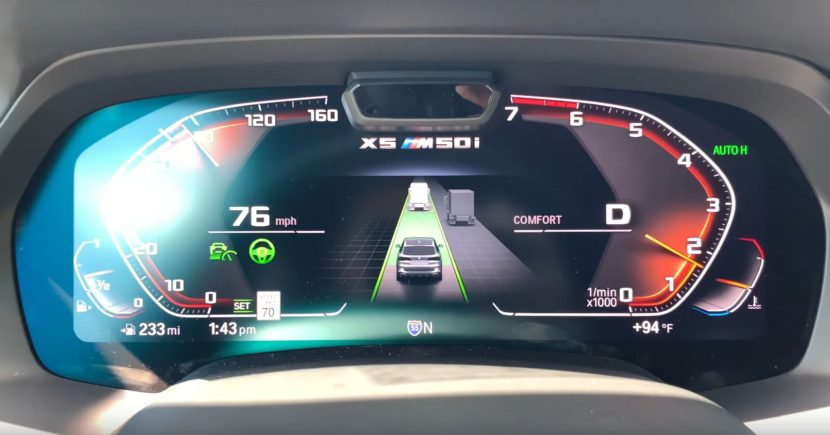
\includegraphics[width=0.7\textwidth]{Figures/bmw.jpg}
	\caption{BMW driving assistent - umiestnenie kamery na snímanie vodiča.\cite{bmw2019assistent}}
	\label{fig:bmwAssistent}
\end{figure}






\newpage
\section{Využitie sférických kamier na detekciu obrazu}
\label{sec:Spherical cameras}

Výstup z kamery je reprezentovaný 2D snímkou, ktorá  zachytáva obraz z celého svojho okolia. Toto zobrazenie sa dá popísať  modelom sférického obrazu (Obr. \ref{fig:sphericalModel}). Predpokladajme, že existuje priestorová guľa a bod \textit{P}, ktorý sa nachádza v priestore. Priesečník povrchu gule s čiarou spájajúcou bod \textit{p} a stred gule je premietanie bodu \textit{p} do gule. Takýmto spôsobom sa získa sférický obraz premietaním všetkých viditeľných bodov do gule. Toto sa nazýva sférická projekcia. Záber sférickej projekcie  môžeme popísať dvomi uhlami. Prvý uhol vyjadruje záber v horizontálnom smere $ \phi \in [-180^\circ , +180^\circ ]$ a druhý uhol vyjadruje záber vo vertikálnom smere  $\theta \in [-90^\circ , +90^\circ ]$.
\begin{figure}[H]
	\centering
	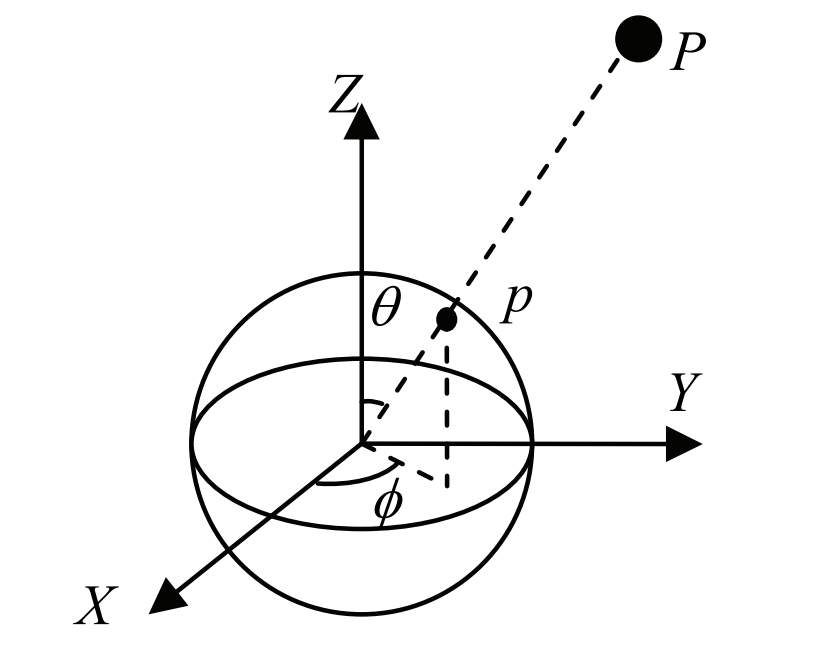
\includegraphics[width=0.5\textwidth]{Figures/sphericalModel.png}
	\caption{Model sférickej projekcie.\cite{li2006full}}
	\label{fig:sphericalModel}
\end{figure}
Zhotovenie takejto sférickej snímky je technicky  náročnjšie ako bežná fotografia. Pre dosiahnutie správneho výsledku je potrebné zachovať určité podmienky. Ideálny sférický model obrazového snímača by mal spĺnať nasledujúce vlastnosti:
\begin{itemize}
\item \textbf{Úplný zorný uhol} \textit{(angl. Full FOV)} - každá sférická kamera by mala vytvárať obraz z celého svojho okolia bez vynechania miesta v scéne. Ak sa nejaká časť scény vynechá, nejedná sa o úplný sfrérický záber.
\item \textbf{Jeden pozorovací zdroj} - snímanie celej scény by malo  byť zabezpečené z jedného rovnakého miesta, aby jednotlivé časti scény na seba správne nadväzovali. V prípade, že by scéna bola snímana z viacerých miest, rekonštrukcia výslednej sférickej sníky  by sa nemusela správne vytvoriť.
\item \textbf{Snímanie celej scény v rovnakom čase} - zariadenie na snímanie by malo vyhotoviť snímok celej scény v jednom momente. Táto vlastnosť je potrebná najmä pri snímaní dynamických scén, alebo pohyblivých objektov. Pri jej nedodržaní by sa pohybujúci objekt mohol vo výslednom obraze objaviť viackrát, alebo byť rozmazaný.
\end{itemize}
\newpage
\subsubsection*{Možnosti snímania sférického obrazu}
Aby  sme dostali obraz, ktorý zachytáva celú scénu, je potrebné takýto obraz najskôr nasmínať. Existuje mnoho metód a postupov, ako možno vytvoriť sférickú fotografiu. Každé riešenie má svoje výhody aj nevýhody, ktoré môžu ovplyvniť konečný výber spôsobu výtvárania sférickej fotografie. Medzi najbežnejšie spôsoby zhotovenia sférických obrazov je možné zaradiť tieto spôsoby:
\begin{itemize}
\item \textbf{Použitie bežného fotoaparátu} - vytvorenie sférickej fotografie je možné aj pomocou  bežného fotoaparátu, ktorý má obmedzený uhol záberu. Aby bolo možné zachytiť celú scnénu, je potrebné  vytvoriť fotografie celej scény, ktoré sa následne poskladajú  do mozaiky. Toto riešenie je veľmi jednoduché, avšak má  obrovské nevýhody. Takýmto  snímaním nie je možné zachytiť dynamickú scénu a na výslednej fotografii sa môžu pohybujúce objekty objaviť viackrát. Ďalšou nevýhodou je zdĺhavé vytváranie a spájanie jednotlivých snímok, ktore nemusia vo výsledku  na seba úplne nadväzovať.

\item \textbf{Použitie skupiny kamier} - riešenie je založené na použití viacerých bežných fotoaparátov súčasne. Takéto zariadenie dokáže v jednom momente ovládať všetky fotoaparáty a zhotoviť fotografiu, ktorú následne správne spojí do výslednej sférickej fotografie. Takéto zariadenie je však technicky náročné a samotné fotoaparáty musia byť schopné komunikovať s hlavnou jednotkou zariadenia. Tento faktor sa vo výsledku prejaví najmä vo vysokej cene zariadennia. Okrem ceny  je však zariadenie veľké a ťažké, čo môže byť pre určité zamerania obmedzujúce. Zariadenie spočívajúce zo skupiny 6 kamier vytvorila napríklad firma GoPro. Skladá sa zo 6 outdoorových kamier, ktoré sú pripojené ku centrálnej jednotke. Ukážky takýchto zariadení sú znázornené na obrázku \ref{fig:goproOmni}

\item \textbf{Použitie všesmerovej kamery} - ďalšiou populárnou metódou je snímať široké scény jediným fotoaparátom s použitím zakriveného zrkadla. Tvar zrkadla môže byť napríklad parabolický, hyperbolicý alebo eliptický, vďaka čomu  poskytuje 360$ ^\circ$ zorné pole v horizontálnej rovine a viac ako 100$^\circ$ vo vertikálnej rovine. Použitie všesmerovej kamery však neprináša  úplný 360$ ^\circ$  obraz celej scény, pretože nieje možné zachytiť  obraz nad šošovkou a obraz pod zakriveným zrkadlom. Z tohto dôvodu môže vzniknúť limitujúci faktor pri výbere.  

\item \textbf{Kombinácia hemisférických kamier} - najpoužívanejšou alternatívou na získanie sférickej fotografie je použitie dvojice objektívov tzv. rybie oko \textit{(angl. Fish eye)}. Takýto objektív sa od obyčajného líši najmä svojím obrovským uhlom záberu, ktorý  mnohokrát prekonáva hranicu 180$ ^\circ$. Samotná sférická kamera sa skladá z dvoch oproti sebe umiestneních objektívov, ktoré sa následne spracujú do výslednej sférickej fotografie. Hlavnou výhodou takétoho riešenia je cena, dostatočne kvalitný obraz bez väčších rozdielov medzi jednotlivými snímkami objektívov a rýchle vytvorenie snímky.

\end{itemize}

\begin{figure}[H]
	\centering
	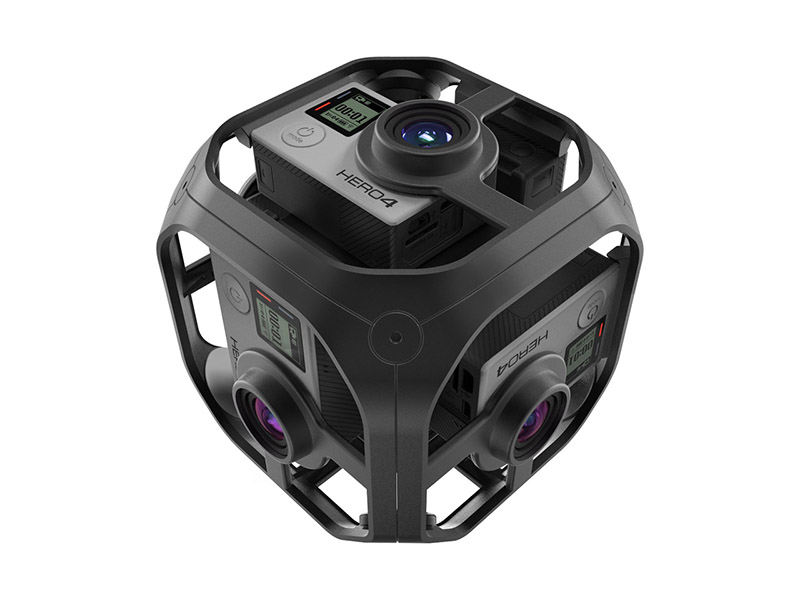
\includegraphics[width=0.3\textwidth]{Figures/goproOmni.jpg}
	\caption{GoPro Omni - séria synchronizovaných kamier pre zachytenie sférickej fotografie.\cite{goproOmni}}
	\label{fig:goproOmni}
\end{figure}


\subsubsection*{Formát sférickej fotografie}
Panoramatické projekcie sa používajú na mapovanie úplnej alebo čiastočnej 3D scény na dvojrozmerný povrch. Napríklad cylindrické projekcie sprostredkujú scénu viditeľnú vo všetkých smeroch, s výnimkou priamo nad kamerou a pod kamerou. To znamená, že horná a dolná časť imaginárneho valca v takýchto obrázkoch máp chýba. Cylindrickú prjekciu je teda možné zobraziť aj ako obyčajnú fotografiu, ktorá však bude veľmi  široká z dôvodu zachytenia scény v celom horizontálnom pásme.
Na rozdiel od cylindrického pohľadu, sférické projekcie majú vertikálny uhol pozorovania 180$ ^\circ$ a horizontálny uhol pohľadu 360$ ^\circ$. Obsahujú svetelné údaje pochádzajúce zo všetkých smerov a preto je možné ich vizualizovať tak, že premietajú jednotlivé body do gule. Medzi najznámejšie  a súčasne používané formáty patria zobrazenie pomocou kubickej mapy \textit{(angl. cubemap)} a ekvidistantné zobrazenie \textit{(angl. equirectangular )}. Tieto projekcie  sa líšia v určitých vlastnostiach:

\begin{itemize}
\item \textbf{Kubické zobrazenie} -  pozostáva zo 6 samostatných plôch kocky na vyplnenie celej scény. Tieto mapy sa často vytvárajú zobrazovaním scény pomocou skupiny šiestich 90-stupňových kamier, ktoré poskytujú textúru vľavo, spredu, vpravo, zozadu, zhora a dole. Šesť obrázkov je zvyčajne usporiadaných ako rozložená kocka. Každá plocha  má zodpovedajúcu textúrnu mapu. Po zložení je pohľad premapovaný na plochy kocky, a pripomínajú kríž položený na bok. Jednotlivé plochy  sa dokážu spojiť veľmi jednoducho. Na jednej strane je kubická projekcia akousi povrchovou textúrou ako obyčajná 2D textúra. Na druhej strane je to určitý formát zobrazenia sférickej fotografie, pretože každý bod v 3D súradnicovom priestore textúry zodpovedá ploche kocky, ku ktorej je najbližšie.

\item \textbf{Ekvidistantné zobrazenie} - tento formát sa stal populárnym v sociálnych sieťach a našiel uplatnenie napríklad v 3D grafických programoch, simuláciách interiérov, panoramatických filmoch či počítačových videohrách. Táto projekcia pozostáva z jedného obrázka v tvare obdĺžnika, ktorého šírka a výška sú v pomere 2: 1. Formát sférickej fotografie je podstatne odlišný od obyčajnej fotografie. Aby bolo možné zachytiť celú priestorovú scénu, je potrebné reprezentovať priestorový záber.
\end{itemize}

\begin{figure}[H]
	\centering
	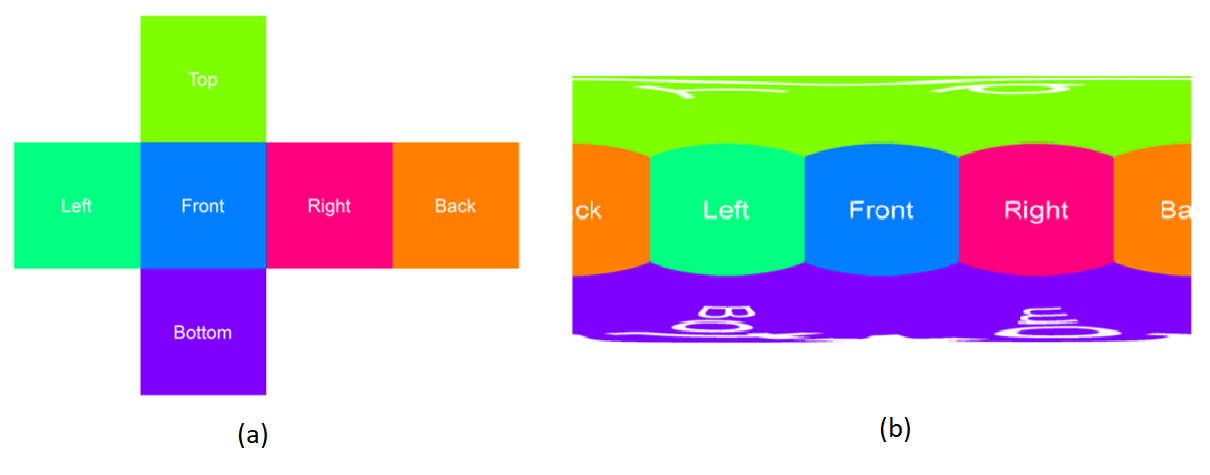
\includegraphics[width=0.9\textwidth]{Figures/sphericalModel2.png}
	\caption{Znázornenie sférických projekcií - kubické zobrazenie (a), ekvidistantné zobrazenie (b)}
	\label{fig:sphericalModel2}
\end{figure}

Konverzia rovnostranného obrázka na kubickú mapu sa najčastejšie používa pre niektoré riešenia virtuálneho prostredia alebo pri úprave severných a južných pólov sférických panorám.
Rovnostranné obrázky sú roztiahnuté v horizontálnom smere. Je to dôvod na značné množstvo redundancie údajov v blízkosti pólov. Pri zmenšovaní obrázka v editore sa efektívne rozlíšenie textúry zníži podľa očakávania - s výnimkou blízkych pólov. To môže spôsobiť radiálne artefakty, ktoré sa zobrazia pri zobrazovaní 3D fotografie. Rovnostranná projekcia je preto vhodná na simuláciu iba tých prostredí, v ktorých sú deformácie textúry v hornej a dolnej časti gule zanedbateľné. Riešením je prepnúť na menej zdeformovanú projekciu pred zmenšením mierky, rozmazaním alebo zaostrením panorámy a v prípade potreby prepnúť do sférického režimu neskôr. Kubická projekmcia našla využitie v počítačovej grafike v reálnom čase. Mapovanie prostredia alebo skôr guľové mapovanie sa používa na vytváranie lesklých alebo reflexných objektov. V takom prípade by textúra mapy mala byť pohľadom na scénu, ktorá sa odráža v lesklej gule.

\begin{figure}[H]
	\centering
	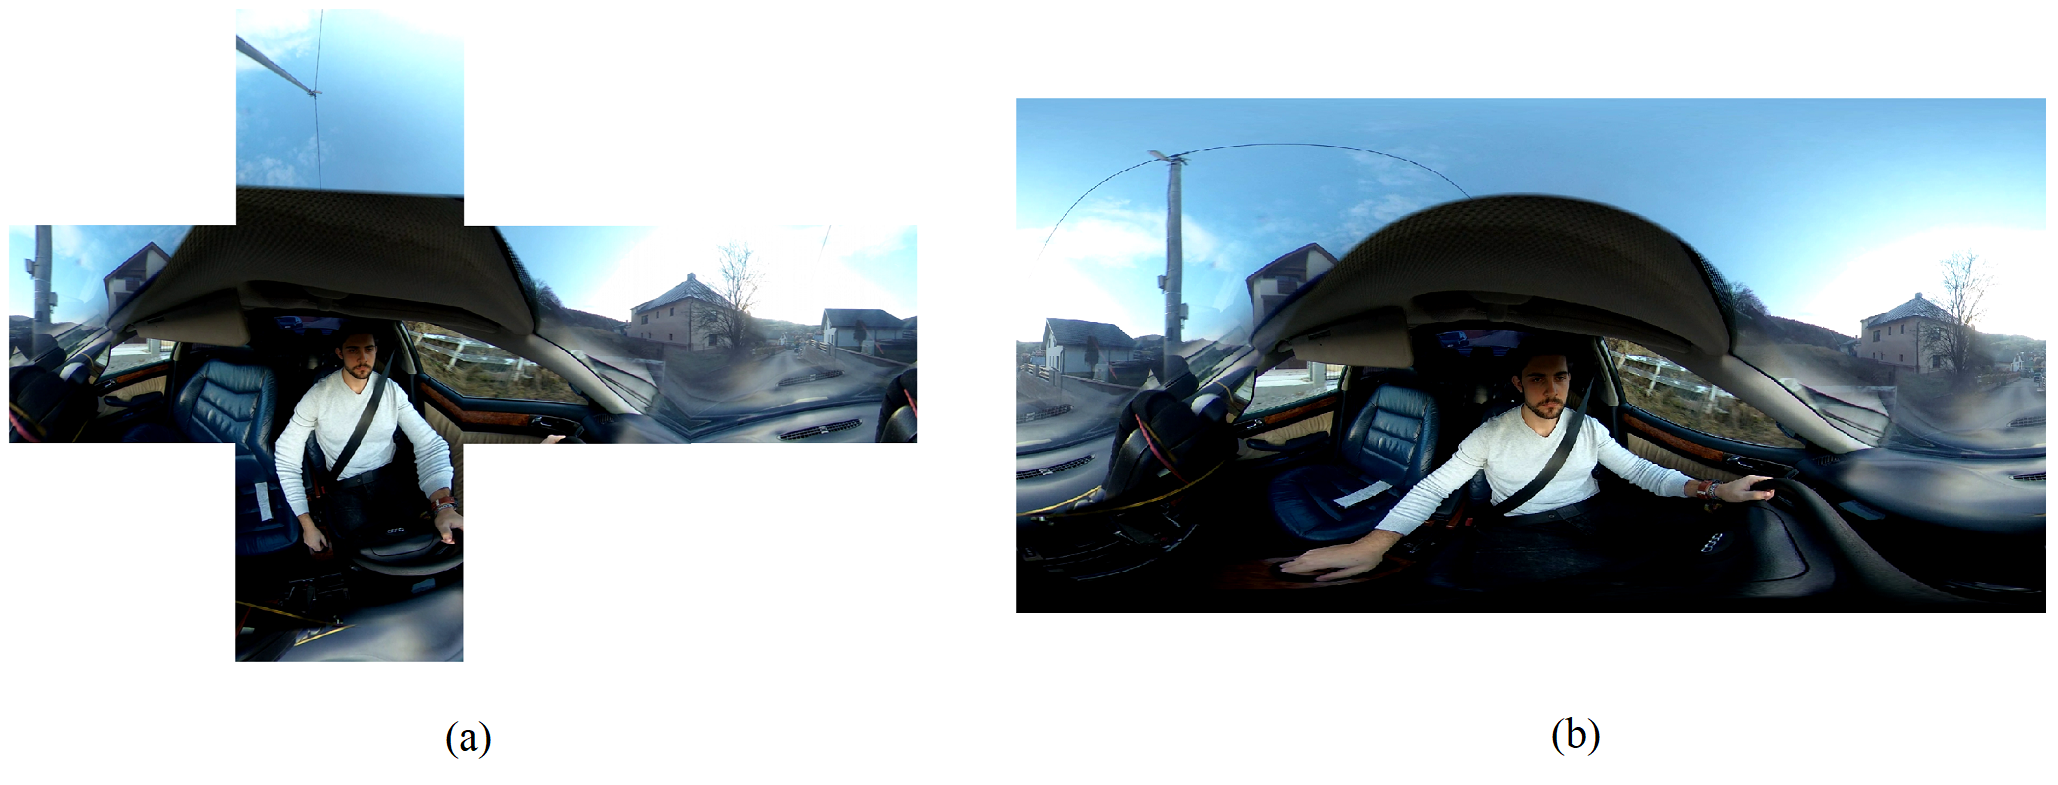
\includegraphics[width=0.9\textwidth]{Figures/cubemapVsEcti.png}
	\caption{Rovnaká sférická fotografia v rôznych zobrazeniach  - kubické zobrazenie (a), ekvidistantné zobrazenie (b)}
	\label{fig:sphereFormats}
\end{figure}




\newpage
\section{Vlastná implementácia}
\label{sec:Vlastná implementácia}

\subsection{Popis programu}
Táto kapitola je zameraná na  popis implementácie vlastného programu. Hlavnou podstatouvýsledného programu je detekcia vodiča z videa alebo z jednotlivých obrázkov nahratých kamerou z interiéru vozidla. V kapitole sú tiež detailné popísané možnosti, problémy a riešenia nahrávania samotných videí z interiéru vozidla pri rôznych problematických podmienkach. Z dôvôdu technickej náročnosti sú tieto videá spracované až dodatočne po ich stiahnutí do počítača, kde sú následne spracované  programom. Riešenie teda neumožňuje spracovanie videa v reálnom čase počas jazdy. To však neznamená, že taká možnosť neexistuje. Tento program môže poslúžiť ako inšpirácia pre budúce riešenia, ktoré by sa zameriavali na spracovanie podobného druhu aj v reálnom čase.\par
Program  by mal byť schopný detekovať vodičove správanie a znázorňovať stav daného vodiča s vyhodnotením situácie. Medzi takúto detekciu patrí napríklad analýza posedu v aute, umiestnenie rúk alebo natočenie hlavy. Program musí podporovať použitie viacerých frameworkov na detekciu ľudských postáv a umožniť porovnanie medzi sebou formou vhodného výstupu. Základné metódy, ktoré musí program podporovať sú Tensorflow pose Estimation a OpenPose. Tieto frameworky boli zvolené najmä z dôvodu, že sa jedná o najviac používanie metódy na detekciu postáv v súčasnosti. Okrem toho majú výborne zdokumentované zdrojové kódy a dostatočné množstvo informácii pre vlastnú implementáciu. Okrem základnej detekcie postáv program umožňuje aj rozšírený mód. Tento rozšírený mód sa zameriava na detekciu ďalších vlastnosti šoféra vozidla ako napríklad zapnutie bezpečnostného pásu, alebo natočenie hlavy. Z týchto informácii je potom možná ďalšia analýza vodičovho správania a vyhodnotenie rizík. Program je rozdelený do jednotlivých samostatných celkov, ktoré sú na sebe nezávislé. Každý z týchto celkov spracováva konkrétnu časť:
\begin{itemize}
\item \textbf{Detekcia vodiča} (Kapitola \ref{sec:driverDetection}) - základným prvkom programu je  analýza vodičovho posedu.  V kapitole je popísané využitie jednotlivých frameworkov na detekciu a analýza ľudského tela zo zozbieraných údajov pomocou jednotlivých frameworkov.

\item \textbf{Otočenie hlavy} (Kapitola \ref{sec:headOrientation}) - je zameraná na rotáciu a natočenie hlavy vodiča pomocou detekcie tvárových landmarkov a knižnice dlib\cite{dlib09}. 

\item \textbf{Bezpečnostný pás} (Kapitola \ref{sec:safeBelt}) - táto kapitola je zameraná  predovšetkým na problematiku snímania bezbečnostného pásu pri rôznych nepriaznivých podmienkach.


\item \textbf{Neurónová sieť} (Kapitola \ref{sec:neuralNetwork}) - vo výslednej časti je popísaná implementácia neurónovej siete, ktorá vyhodnocuje jednotlivé výstupy predchádzajúcich častí.

\end{itemize}

\newpage
\subsection{Požiadavky a návrh programu}
Každý vyvíjaný program, by mal  spĺnať určité očakávania. Tieto očakávania a požiadavky by mali byť správne zadefinované ešte samotným vývojom. Tieto požiadavky okrem toho, že určia samotnú funkcionalitu programu, zároveň umožňujú analyzovať splnenie jednotlivých bodov. Požiadavky by mali byť priebežne spracované. Pri správnej analýze ešte pred samotným vývojom programu je potom jednoduché kontrolovať splnenie jednotlivých bodov. Program, ktorý je navrhnutý v tejto diplomovej práci obsahuje niekoľko dôležitých podmienok, ktoré zaručia dostatočnú kvalitu výstupu programu a jeho použitie. Jednotlivé požiadavky sú zhrnuté v nasledujúcich bodoch:
\begin{itemize}
\item \textbf{Jednoduché používanie} - program  musí byť jednoduchý na používanie. To znamená, že by mal obsahovať  iba určitú funkcionalitu, ktorej výsledok je požadovaný a zrejmý. Ku programu by mala byť zároveň vytvorená jednoduchá dokumentácia, ktorá by obsahovala jednotlivé príkazy a popis parametrov.

\item \textbf{CLI podpora} - pre univerzálnosť použitia by mal program byť spustitelný z príkazového riadku. Jednotlivé časti programu by mali byť jednoducho používané pomocou voliteľných parametrov.

\item \textbf{Nezávislosť na použitej kamere} - program by  mal byť schopný spracovať  akékoľvek video, ktoré bude nahraté z interiéru vozidla. Nemal by byť závislý na formáte, ani type samotných videí.

\item \textbf{Podpora  viacerých frameworkov na detekciu postáv} - program musí podporovať aspoň 2 rôzne frameworky, ktoré slúžia na detekciu postáv v obraze.Ich  použitie by nemalo byť závislé na type videa alebo použití inej funkcionality. Táto podmienka vyžaduje zjednotenie vstupov a výstupov pre jednotlivé frameworky na detekciu postáv v obraze.
\item \textbf{Znázornenie výsledku detekcie} - pre program by mal umožnovať výpis jednotlivých časti programov priamo do obrazu.
\item \textbf{Štatistické údaje} - program by po svojom úspešnom skončení mal byť schopný  zozbierať a vyhodnotiť údaje z celeho behu programu. Dôležité údaje sú čas spracovania jednej snímky, celková úspešnosť a celková doba programu. 
\item \textbf{Univerzálnosť} -  aby bolo jednoduché použiť program na viacerých operačných systémov, je potrebné ho napísať tak, aby  nevyužíval žiadnu funkconalitu, ktorá je závisla na konkrétnom operačnom systéme. 
\end{itemize}

\newpage
\subsection{Použité technológie}

\subsubsection*{Programovací jazyk}
Hlavný program je napísaný v jazyku Python. Tento jazyk bol použitý z dôvodu výnikajúcej dostupnosti knižníc na spracovanie obrazu, ale aj knižníc na prácu s neurónovými sieťami. Okrem toho je jazyk Python veľmi dobre zdokumentovaný a má vybudovanú širokú komunitu medzi programátormi. Okrem jazyka Python taktiež bolo zvažované použitie jazyka C++.  Napriek mnohým nesporným výhodam jazyka C++ padlo rozhodnutie pre jazyk Python najmä po dôkladnom zvážení nasledujúcich možností:
\begin{itemize}
\item \textbf{Automatická správa pamäte} - Python má narozdiel od C++  implicitne  vyriešenú automatickú alokáciu a dealokáciu pamäte. To dáva programátorovi výhodu v ušetrení času za cenu malého zníženia výkonu aplikácie.
\item \textbf{Široká podpora knižníc} - v súčasnosti pre jazyk Python existuje obrovské množstvo voľne dostupných knižníc, ktoré uľahčujú prácu pri vývoji softvéru. Jedná sa najmä o knižnice zamerané na prácu s neuronovými sieťamia spracovanie obrazu.
\item \textbf{Jednoduchosť jazyka} - Python je narozdiel od C++ jednoduchší a pohodlnejší  na používanie. Poskytuje mnohé výhody, ktoré jazyk C++ nepodporuje ako napríklad dynamické dátové typy, jednoduchá inštalácia a použitie potrebných baličkov v programe.
\end{itemize}

\subsubsection*{OpenCV}
OpenCV je multiplatformová knižnica, ktorá obsahuje funkcie pre spracovanie a manipuláciu s obrazom v reálnom čase. Vďaka licencii BSD je možné používáť OpenCV zadarmo  nielen pre akademické, ale aj pre komerčné účely. S jej využitím je možné sa stretnúť pri analýze a spracovanie snímok z rôznych oblastí. Aplikácie, ktoré sú napísané a optimalizované v C/C++, potom môžu pre svoj beh využívať viacjadrové procesory. V súčasnosti sa výrazne rozšírila podpora aj pre jazyk Python a CUDA pre spracovanei na grafickom procesore. V programe je OpenCV využité  na základnú prácu s obrazmi ako načítanie snímky z videa, zmena veľkosti, detekcia hrán a podobne.


\subsubsection*{TensorFlow}
TensorFlow\cite{tensorflow2015-whitepaper} bol pôvodne vyvinutý výskumníkmi a inžiniermi pracujúcimi v tíme Google Brain v rámci organizácie Google Research Intelligence Research na vykonávanie strojového učenia a výskumu neurónových sietí. Framework je dostatočne všeobecný na to, aby sa dal použiť aj v mnohých ďalších doménach. TensorFlow poskytuje stabilné API  pre jazyky Python a C++, ako aj nezaručené kompatibilné API pre iné jazyky. V programe je Tensorflow využitý najmä na detekciu postáv a prácu s neuronovými sieťami.



\subsubsection*{Keras}
Keras\cite{chollet2015keras} je framework pre hĺbkové učenie pôvodne vyvinutý pre jazyk Python. Poskytuje pohodlný spôsob, ako definovať a trénovať takmer akýkoľvek druh hlbokého učenia. Keras je vysokoúrovňové API pre neurónové siete, ktoré je schopné pracovať s inými knižnicami ako napríklad nad Tensorflow, Theano\cite{theano} a CNTK. V aplikácii je Keras využitý na vytvorenie modelu a jednotlivých vrstiev neurónovej siete.



\subsection{Vytvorenie a spracovanie videa}
V tejto sekcii je postupne spísaný postup a problematika, ktorá sa týka nahrávania videí potrebných pre analýzu vodiča v tejto diplomovej práci. Samotný program je pôvodne navrhnutý na spracovanie videa v 360 stupňovom formáte. Implementácia však nie je žiadnym spôsobom limitovaná a program je schopný spracovať aj obyčajné video nahraté bežne dostupnou kamerou. Hlavným dôvôdom použitia  sférickej kamery je jej uhol záberu. Vďaka širokouhlému obrazu je možné získať obraz celého vodiča sediaceho za volantom. Získanie takéhoto obrazu umožňuje analyzovať jednotlivé časti tela, tvár, ale aj vodičovo správanie.\par
 Počas vypracovania práce boli k dispozícii dve širokouhlé kamery od rôznych výrobcov. Na kamerách je umiestnené minimálne množstvo tlačidiel, ktoré slúžia prímárne iba na zapnutie a vypnutie kamery. Celé ovládanie je cez intuitívne mobilné aplikácie, ktoré sú dostupné na stiahnutie na stránkach výrobcov pre všetky mobilné platformy používané v súčasnosti. Obidve kamery obsahujú 2 objektivy tzv. fish eye, s ktorými sa vytvára sférický záber okolitej scény. Kamery majú odlišné parametre a vlastnosti, ktoré sú zhrnuté v tabuľke \ref{tab:techSpec}. Hlavný rozdiel je možné vidieť najmä v maximálnom rozlíšení, ktoré je pri videu pre kameru GoPro Fusion takmer dvojnásobné oproti rozlíšeniu kamery Ricoh Theta V. Pri spracovaní videa a detekcii vodiča však nemusí rozlíšenie hrať významnú úlohu. Pri detekcii objektov sférickou kamerou zhorávajú úlohu aj ostatné parametre ako napríklad svetelnsoť použitých senzorov.

\begin{table}[H]
\begin{tabular}{|l|c|c|}
\hline
                                     & \textbf{GoPro Fusion}  & \textbf{Ricoh Theta V} \\ \hline
\textbf{Senzor}                      & FishEye CMOS 2×18MP    & FishEye CMOS 2×12MP    \\ \hline
\textbf{Max. rozlíšenie (foto)}      & 18MP                   & 14.4MP                 \\ \hline
\textbf{Max. rozlíšenie (video)}     & 13.7MP                 & 7.3MP                  \\ \hline
\textbf{Sveteľnosť senzora}          &  f/2.0                 & f/2.0                  \\ \hline
\textbf{Pamäť}                       &  SD karta (256GB)      & 19GB                   \\ \hline
\end{tabular}

	\caption{Technické parametre sférických kamier}
	\label{tab:techSpec}
\end{table}
\newpage
 Hlavný rozdiel je možné vidieť najmä v maximálnom rozlíšení, ktoré je pri videu pre kameru GoPro Fusion takmer dvojnásobné oproti rozlíšeniu kamery Ricoh Theta V. Pri spracovaní videa a detekcii vodiča však nemusí rozlíšenie hrať významnú úlohu. Pri detekcii objektov sférickou kamerou zhorávajú úlohu aj ostatné parametre ako napríklad svetelnsoť použitých senzorov. Aj napriek tomu, že svetelnosť senzora je totožná pri obidvoch kamerách, rozdiel v kvalite výstupného videa je ľahko rozpoznateľný najmä pri znížených svetelných podmienkach. Kým za denného svetla sú kvalita aj kontrast obrazu skoro totožné pre obidve kamery, pri tmavých scénach je obraz z kamery Ricoh Theta V nekvalitný a obsahuje vysokú úroveň šumu za cenu vyššej priepustnosti svetelnosti (Obr. \ref{fig:cameraCompare}). Pri natáčaní tmavých scén bolo použité na obidvoch kamerách ISO 1600. Napriek rovnakým nastaveniam je z obrázku vidieť, že výstup z kamery GoPro Fusion je značne tmavší. Na tomto obrázku zároveň vidieť problém, ktorý nastáva  pri znížených svetelných podmienkach. Keďže ani jedna kamera nie je vybavená infračerveným svetlom, ktoré by pomáhalo v noci, detekcia kamerou  nie je veľmi účinná. Svetelnosť scény je možné upraviť zvýšenim ISO ale za cenu vyššieho šumu v obraze. Z tohto dôvodu bolo na kamerých nastavené vždy autoamtické ISO, ktoré sa prispôsobovalo okolitým svetelným podmienkam. Hlavne z tohto dôvôdu väčšinou prebiehal zber záberov počas denného svetla. Pri  použití kamery v noci by bolo potrebné nájsť rozumný spôsob, ako scénu nasvetliť aby postava vodiča bola vidideľná. Pri spracovaní videí z obidvoch kamier, bolo používané iba video z prednej kamery. Pre potreby tejto práce bol potrebný záber celého tela vodiča za volantom. Z dôvôdu, že táto práca je zameraná iba na detekciu vodiča je záber jedným objektívom postačujúci a nemá zmysel spracovávať výstup z druhého objektívu. Takýmto spôsobom bolo vytvorených približne 15 minút záznamov z každej kamery v rôznych podmienkach.

\begin{figure}[H]
	\centering
	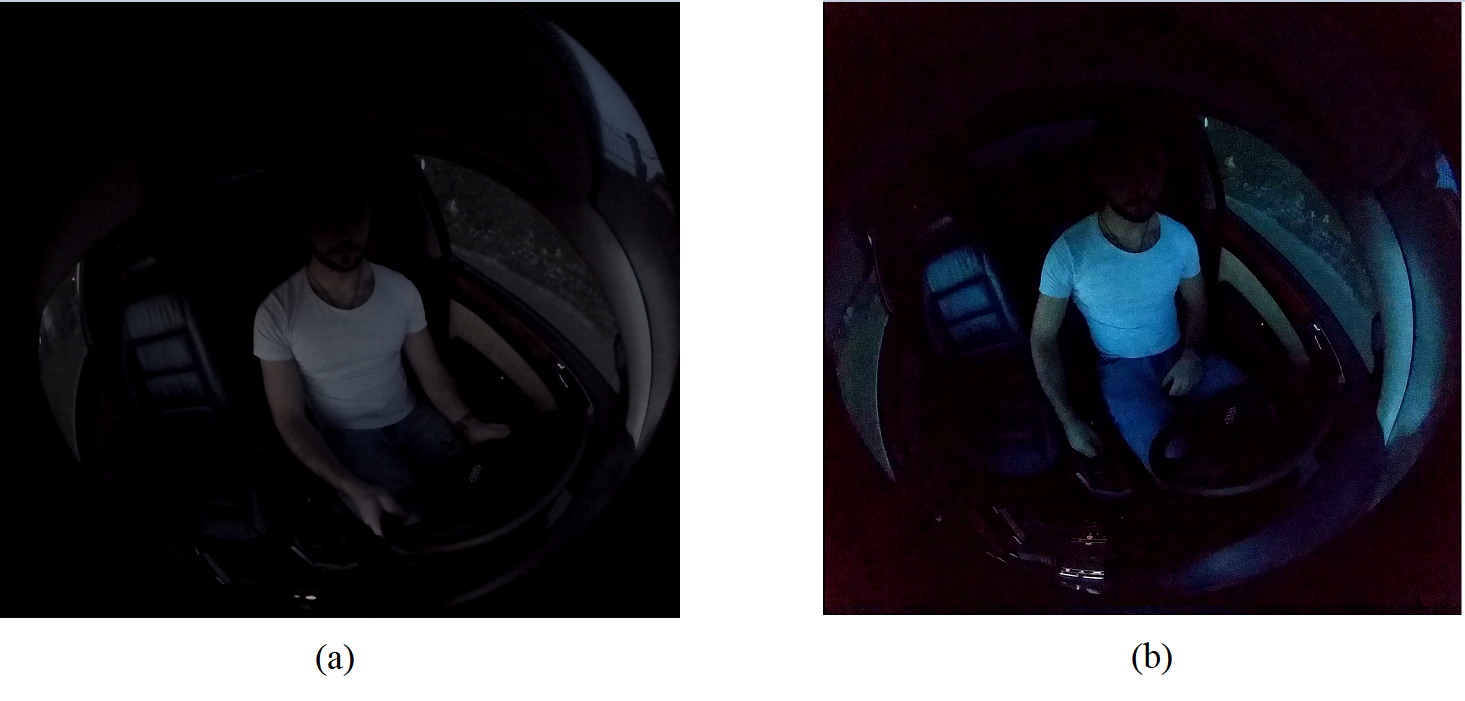
\includegraphics[width=1\textwidth]{Figures/camCompare.png}
	\caption{Porovnanie výstupu z kamier (ISO 1600) - GoPro Fusion(a), Ricoh Theta V(b)}
	\label{fig:cameraCompare}
\end{figure}



\newpage
\subsection{Detekcia vodiča}
\label{sec:driverDetection}
Po úspešnom vytvorení testovacích videí prichádza na rad detekcia vodiča. Pred samotnou detekciou je nutné video najskôr upraviť, aby bolo podľa možnosti v čo najvhodnejšej forme pre jednotlivé frameworky. Dôležitá úprava, ktorú je potrebné urobiť je zmena rozlíšenia. Všetky frameworky na detekciu postáv v obrazoch pracujú odlišne vzhľadom na zvolené rozlíšenie. Úpravou rozlíšenia je tiež možné možné ľahšie testovať a hľadať najvhodnejšie parametre pre dosiahnutie  najvyššej úspešnosti. Na úpravu rozlíšenia je vytvorená funkcia, ktorá na základe požadovanej výšky  snímky  zmení veľkosť  snímky tak, aby bol zachovaný správny pomer strán. Tým je zabezpečené, že obraz nebude žiadnym spôsobom deformovaný a výsledné rozlíšenie je ľahko nastaviteľné. Táto funkcia bude využívaná aj v ďalších častiach práce.\par
Obidva použité frameworky pracujú na odlišných princípoch. Preto bolo potrebné naštudovanie dokumentácie a príprava implementácie. Okrem toho používajú odlišné datasety, ktoré sa dajú parametrizovať a vybrať ten najvhodnejší. Každý framework  vyžaduje správny postup krokov pre použitie vo vývojárskom prostredí. Po správnej inštálácii vštkých potrebných knižníc a balíčkov  je potrebné ich správne nakonfigurovať. Openpose ponúka na výber mnoho parametrov. Jedným z dôležitých parametrov pri detekcii postáv v obraze je použitý dataset.

\subsubsection*{OpenPose}
 Pri implementácii OpenPose bol použitý dataset MPI a dataset COCO. Výber datasetu je možný cez parameter. Openpose podporuje aj použitie moderného a presnejšieho datasetu BODY\_25, avšak z dôvodu nepostačujúceho výpočtového výkonu nebol v tejto práci používaný.// TODO

\subsubsection*{TF Pose}
- TODO


\subsubsection*{Zjednotenie výstupov}
- TODO
- fasada\\
- graf


\newpage
\lstinputlisting[label=src:poseUnifier,caption={Mapovanie častí ľudského tela rôznych frameworkov}]{SourceCodes/poseUnifier.py}
 
\newpage
\subsection{Orientácia hlavy}
\label{sec:headOrientation}
- Haar  priznaky ,\\
- prevod 2D na 3D \\
- smerova priamka

\newpage
\subsection{Bezpečnostný pás}
\label{sec:safeBelt}
- bezp. pas

\newpage
\subsection{Neurónová sieť}
\label{sec:neuralNetwork}
-NN klasifikator\\
- trenovanie \\
- testovanie

\newpage
\subsection{Výstup programu}
obrazky\\
tabulky

\newpage
\subsection{Porovnanie výsledkov}
porovnanie


\newpage
\subsection{Využitie zozbieraných dát}
pouzitie v buducnosti


\newpage
\subsection{Používateľská príručka}
python program.py --use-openPose=true


\newpage
\section{Možnosti vylepšenia detekcie}
\label{sec:Možnosti vylepšenia detekcie}
Zhrnutie vysledkov


\newpage
\section{Záver}
\label{sec:Zaver}
Zhrnutie vysledkov







\bibliography{literatura}














\end{document}
